\let\negmedspace\undefined
\let\negthickspace\undefined
\documentclass[journal,12pt,onecolumn]{article}
\usepackage{cite}
\usepackage{amsmath,amssymb,amsfonts,amsthm}
\usepackage{algorithmic}
\usepackage{graphicx}
\usepackage{textcomp}
\usepackage{xcolor}
\usepackage{txfonts}
\usepackage{listings}
\usepackage{enumitem}
\usepackage{mathtools}
\usepackage{gensymb}
\usepackage{comment}
\usepackage[breaklinks=true]{hyperref}
\usepackage{tkz-euclide} 
\usepackage{listings}
\usepackage{gvv}                                        
%\def\inputGnumericTable{}                                 
\usepackage[latin1]{inputenc}     
\usepackage{xparse}
\usepackage{color}                                            
\usepackage{array}                                            
\usepackage{longtable}                                       
\usepackage{calc}                                             
\usepackage{multirow}
\usepackage{multicol}
\usepackage{hhline}                                           
\usepackage{ifthen}                                           
\usepackage{lscape}
\usepackage{tabularx}
\usepackage{array}
\usepackage{float}
\usepackage{bm}
\newtheorem{theorem}{Theorem}[section]
\newtheorem{problem}{Problem}
\newtheorem{proposition}{Proposition}[section]
\newtheorem{lemma}{Lemma}[section]
\newtheorem{corollary}[theorem]{Corollary}
\newtheorem{example}{Example}[section]
\newtheorem{definition}[problem]{Definition}
\newcommand{\BEQA}{\begin{eqnarray}}
\newcommand{\EEQA}{\end{eqnarray}}
\usepackage{float}
%\newcommand{\define}{\stackrel{\triangle}{=}}
\theoremstyle{remark}
\usepackage{ circuitikz }
%\newtheorem{rem}{Remark}
% Marks the beginning of the document
\begin{document}

\title{CE - 2021}
\author{EE25BTECH11043 - Nishid Khandagre}
\date{}
\maketitle

\renewcommand{\thefigure}{\theenumi}
\renewcommand{\thetable}{\theenumi}

\textbf{SESSION -1}
\section*{Q.1 - Q.5 Multiple Choice Question}
\begin{enumerate}
\item Getting to the top is \underline{\hspace{2cm}} than staying on top.

\hfill{\brak{\text{GATE CE 2021}}}
\begin{enumerate}
\begin{multicols}{4}
    \item more easy
    \item much easy
    \item easiest
    \item easier
\end{multicols}
\end{enumerate}

\item The mirror image of the above text about the X-axis is
\begin{figure}[H]
        \centering
        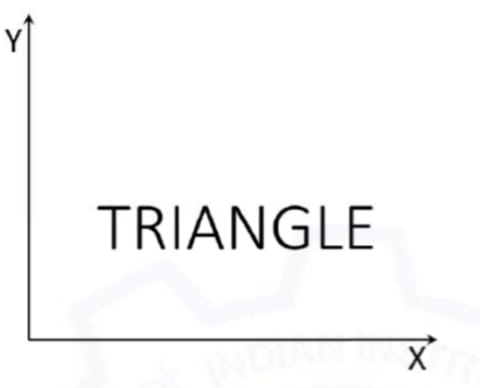
\includegraphics[width=0.7\columnwidth]{figs/1q2.jpg}
        \caption{}
        \label{fig:2}
    \end{figure}
\hfill{\brak{\text{GATE CE 2021}}}
\begin{multicols}{2}
\begin{enumerate}
    \item 
    \begin{figure}[H]
        \centering
        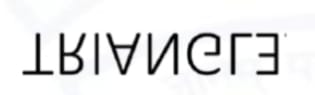
\includegraphics[width=0.7\columnwidth]{figs/1q2a.jpg}
        \caption{}
        \label{fig:a2A}
    \end{figure}
    \item 
    \begin{figure}[H]
        \centering
        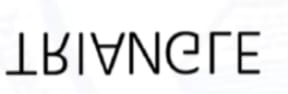
\includegraphics[width=0.7\columnwidth]{figs/1q2b.jpg}
        \caption{}
        \label{fig:a2B}
    \end{figure}
    \item 
    \begin{figure}[H]
        \centering
        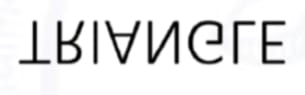
\includegraphics[width=0.7\columnwidth]{figs/1q2c.jpg}
        \caption{}
        \label{fig:a2C}
    \end{figure}
    \item 
    \begin{figure}[H]
        \centering
        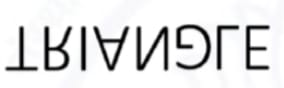
\includegraphics[width=0.7\columnwidth]{figs/1q2d.jpg}
        \caption{}
        \label{fig:a2D}
    \end{figure}
\end{enumerate}
\end{multicols}

\item In a company, $35\%$ of the employees drink coffee, $40\%$ of the employees drink tea and $10\%$ of the employees drink both tea and coffee. What $\%$ of employees drink neither tea nor coffee?

\hfill{\brak{\text{GATE CE 2021}}}
\begin{enumerate}
\begin{multicols}{4}
    \item $15$
    \item $25$
    \item $35$
    \item $40$
\end{multicols}
\end{enumerate}

\item $\oplus$ and $\odot$ are two operators on numbers $p$ and $q$ such that
\begin{align}
p \oplus q = \frac{p^2+q^2}{pq} \quad \text{and} \quad p \odot q = \frac{p^2}{q}
\end{align}
If $x \oplus y = 2 \odot 2$, then $x =$

\hfill{\brak{\text{GATE CE 2021}}}
\begin{enumerate}
\begin{multicols}{2}
    \item $\frac{y}{2}$
    \item $y$
    \item $\frac{3y}{2}$
    \item $2y$
\end{multicols}
\end{enumerate}

\item Four persons P, Q, R and S are to be seated in a row, all facing the same direction, but not necessarily in the same order. P and R cannot sit adjacent to each other. S should be seated to the right of Q. The number of distinct seating arrangements possible is:

\hfill{\brak{\text{GATE CE 2021}}}
\begin{enumerate}
\begin{multicols}{4}
    \item $2$
    \item $4$
    \item $6$
    \item $8$
\end{multicols}
\end{enumerate}

\item Statement: Either P marries Q or X marries Y

Among the options below, the logical NEGATION of the above statement is:

\hfill{\brak{\text{GATE CE 2021}}}
\begin{enumerate}
    \item P does not marry Q and X marries Y.
    \item Neither P marries Q nor X marries Y.
    \item X does not marry Y and P marries Q.
    \item P marries Q and X marries Y.
\end{enumerate}

\item Consider two rectangular sheets, Sheet M and Sheet N of dimensions $6cm \times 4cm$ each.

Folding operation 1: The sheet is folded into half by joining the short edges of the current shape.

Folding operation 2: The sheet is folded into half by joining the long edges of the current shape.

Folding operation 1 is carried out on Sheet M three times.
Folding operation 2 is carried out on Sheet N three times.
The ratio of perimeters of the final folded shape of Sheet N to the final folded shape of Sheet M is \underline{\hspace{2cm}}.

\hfill{\brak{\text{GATE CE 2021}}}
\begin{enumerate}
\begin{multicols}{2}
    \item $13:7$
    \item $3:2$
    \item $7:5$
    \item $5:13$
\end{multicols}
\end{enumerate}


\item Five line segments of equal lengths, PR, PS, QS, QT and RT are used to form a star as shown in the figure \figref{fig:q8} above.
The value of $\theta$, in degrees, is \underline{\hspace{2cm}}
\begin{figure}[H]
    \centering
    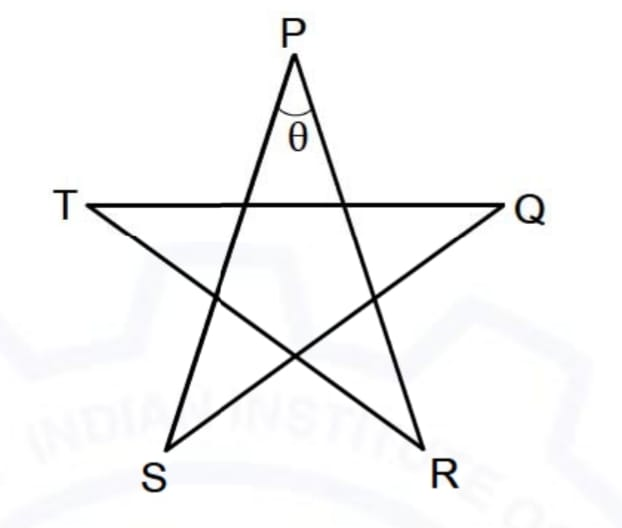
\includegraphics[width=0.7\columnwidth]{figs/1q8.jpg}
    \caption{}
    \label{fig:q8}
\end{figure}
\hfill{\brak{\text{GATE CE 2021}}}
\begin{enumerate}
\begin{multicols}{2}
    \item $36$
    \item $45$
    \item $72$
    \item $108$
\end{multicols}
\end{enumerate}

\item A function, $\lambda$, is defined by
\begin{align}
\lambda\brak{p,q} = 
\begin{cases}
    \brak{p-q}^2, & \text{if } p \geq q, \\
    p+q, & \text{if } p < q.
\end{cases}
\end{align}
The value of the expression $\frac{\lambda\brak{-\brak{-3+2}, \brak{-2+3}}}{\brak{-\brak{-2+1}}}$ is:

\hfill{\brak{\text{GATE CE 2021}}}
\begin{enumerate}
\begin{multicols}{2}
    \item $-1$
    \item $0$
    \item $\frac{16}{3}$
    \item $16$
\end{multicols}
\end{enumerate}

\item Humans have the ability to construct worlds entirely in their minds, which don't exist in the physical world. So far as we know, no other species possesses this ability. This skill is so important that we have different words to refer to its different flavors, such as imagination, invention and innovation.
Based on the above passage, which one of the following is TRUE?

\hfill{\brak{\text{GATE CE 2021}}}
\begin{enumerate}
    \item No species possess the ability to construct worlds in their minds.
    \item The terms imagination, invention and innovation refer to unrelated skills.
    \item We do not know of any species other than humans who possess the ability to construct mental worlds.
    \item Imagination, invention and innovation are unrelated to the ability to construct mental worlds.
\end{enumerate}
\end{enumerate}

\begin{enumerate}
\section*{Q.1 - Q.16 Multiple Choice Question}

\item The rank of matrix $\myvec{1 & 2 & 2 & 3 \\ 3 & 4 & 2 & 5 \\ 5 & 6 & 2 & 7 \\ 7 & 8 & 2 & 9}$ is

\hfill{\brak{\text{GATE CE 2021}}}
\begin{enumerate}
\begin{multicols}{4}
    \item $1$
    \item $2$
    \item $3$
    \item $4$
\end{multicols}
\end{enumerate}

\item If $P = \myvec{1 & 2 \\ 3 & 4}$ and $Q = \myvec{1 & 0 \\ 0 & 1}$ then $Q^T P^T$ is

\hfill{\brak{\text{GATE CE 2021}}}
\begin{enumerate}
\begin{multicols}{2}
    \item $\myvec{1 & 3 \\ 2 & 4}$
    \item $\myvec{1 & 2 \\ 3 & 4}$
    \item $\myvec{2 & 1 \\ 4 & 3}$
    \item $\myvec{2 & 4 \\ 1 & 3}$
\end{multicols}
\end{enumerate}

\item The shape of the cumulative distribution function of Gaussian distribution is

\hfill{\brak{\text{GATE CE 2021}}}
\begin{enumerate}
    \item Horizontal line
    \item Straight line at $45$ degree angle
    \item Bell-shaped
    \item S-shaped
\end{enumerate}

\item A propped cantilever beam EF is subjected to a unit moving load as shown in the figure \figref{fig:q4} \brak{\text{not to scale}}. The sign convention for positive shear force at the left and right sides of any section is also shown.
\begin{figure}[H]
    \centering
    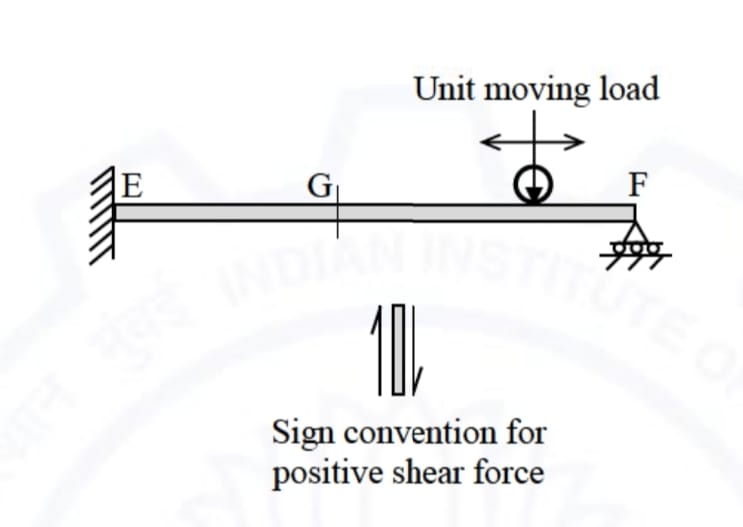
\includegraphics[width=0.7\columnwidth]{figs/1q4.jpg}
    \caption{}
    \label{fig:q4}
\end{figure}
The CORRECT qualitative nature of the influence line diagram for shear force at G is

\hfill{\brak{\text{GATE CE 2021}}}
\begin{enumerate}
  \item \begin{figure}[H]
    \centering
    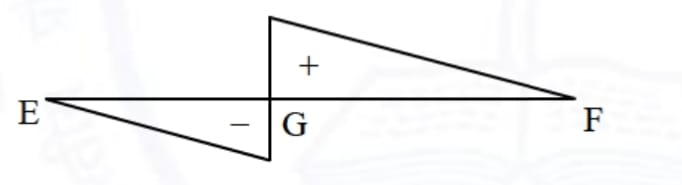
\includegraphics[width=0.7\columnwidth]{figs/1q4a.jpg}
    \caption{}
    \label{fig:q4}
\end{figure}
  \item \begin{figure}[H]
    \centering
    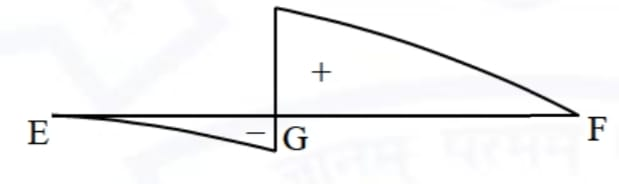
\includegraphics[width=0.7\columnwidth]{figs/1q4b.jpg}
    \caption{}
    \label{fig:q4}
\end{figure}
  \item \begin{figure}[H]
    \centering
    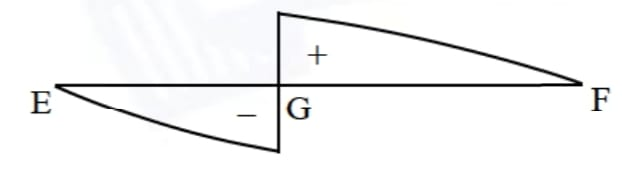
\includegraphics[width=0.7\columnwidth]{figs/1q4c.jpg}
    \caption{}
    \label{fig:q4}
\end{figure}
  \item \begin{figure}[H]
    \centering
    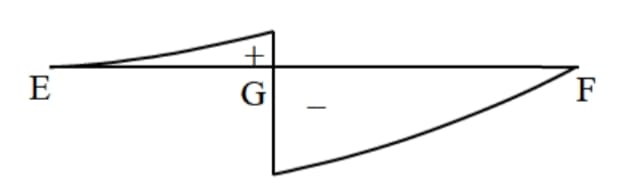
\includegraphics[width=0.7\columnwidth]{figs/1q4d.jpg}
    \caption{}
    \label{fig:q4}
\end{figure}
\end{enumerate}

\item Gypsum is typically added in cement to

\hfill{\brak{\text{GATE CE 2021}}}
\begin{enumerate}
\begin{multicols}{2}
    \item prevent quick setting
    \item enhance hardening
    \item increase workability
    \item decrease heat of hydration
\end{multicols}
\end{enumerate}

\item The direct and indirect costs estimated by a contractor for bidding a project is Rs.160000 and Rs.20000 respectively. If the mark up applied is $10\%$ of the bid price, the quoted price in Rs of the contractor is

\hfill{\brak{\text{GATE CE 2021}}}
\begin{enumerate}
\begin{multicols}{2}
    \item $200000$
    \item $198000$
    \item $196000$
    \item $182000$
\end{multicols}
\end{enumerate}

\item In an Oedometer apparatus, a specimen of fully saturated clay has been consolidated under a vertical pressure of 50 kN/m$^2$ and is presently at equilibrium. The effective stress and pore water pressure immediately on increasing the vertical stress to 150 kN/m$^2$, respectively are

\hfill{\brak{\text{GATE CE 2021}}}
\begin{enumerate}
\begin{multicols}{2}
    \item 150 kN/m$^2$ and $0$
    \item 100 kN/m$^2$ and 50 kN/m$^2$
    \item 50 kN/m$^2$ and 100 kN/m$^2$
    \item $0$ and 150 kN/m$^2$
\end{multicols}
\end{enumerate}

\item A partially-saturated soil sample has natural moisture content of $25\%$ and bulk unit weight of 18.5 kN/m$^3$. The specific gravity of soil solids is 2.65 and unit weight of water is 9.81 kN/m$^3$. The unit weight of the soil sample on full saturation is

\hfill{\brak{\text{GATE CE 2021}}}
\begin{enumerate}
\begin{multicols}{2}
    \item 21.12 kN/m$^3$
    \item 19.03 kN/m$^3$
    \item 20.12 kN/m$^3$
    \item 18.50 kN/m$^3$
\end{multicols}
\end{enumerate}

\item If water is flowing at the same depth in most hydraulically efficient triangular and rectangular channel sections then the ratio of hydraulic radius of triangular section to that of rectangular section is

\hfill{\brak{\text{GATE CE 2021}}}
\begin{enumerate}
\begin{multicols}{2}
    \item $\frac{1}{\sqrt{2}}$
    \item $\sqrt{2}$
    \item $1$
    \item $2$
\end{multicols}
\end{enumerate}

\item 'Kinematic viscosity' is dimensionally represented as

\hfill{\brak{\text{GATE CE 2021}}}
\begin{enumerate}
\begin{multicols}{2}
    \item $\frac{M}{LT}$
    \item $\frac{M}{L^2T}$
    \item $\frac{T^2}{L}$
    \item $\frac{L^2}{T}$
\end{multicols}
\end{enumerate}

\item Which one of the following statements is correct?

\hfill{\brak{\text{GATE CE 2021}}}
\begin{enumerate}
    \item Pyrolysis is an endothermic process, which takes place in the absence of oxygen.
    \item Pyrolysis is an exothermic process, which takes place in the absence of oxygen.
    \item Combustion is an endothermic process, which takes place in the abundance of oxygen.
    \item Combustion is an exothermic process, which takes place in the absence of oxygen.
\end{enumerate}

\item Which one of the following is correct?
\hfill{\brak{\text{GATE CE 2021}}}
\begin{enumerate}
    \item The partially treated effluent from a food processing industry, containing high concentration of biodegradable organics, is being discharged into a flowing river at a point P. If the rate of degradation of the organics is higher than the rate of aeration, then dissolved oxygen of the river water will be lowest at point P.
    \item The most important type of species involved in the degradation of organic matter in the case of activated sludge process based wastewater treatment is chemoheterotrophs.
    \item For an effluent sample of a sewage treatment plant, the ratio $\text{BOD}_{5\text{-day},20\degree C}$ upon ultimate BOD is more than $1$.
    \item A young lake characterized by low nutrient content and low plant productivity is called eutrophic lake.
\end{enumerate}

\item The liquid forms of particulate air pollutants are

\hfill{\brak{\text{GATE CE 2021}}}
\begin{enumerate}
\begin{multicols}{2}
    \item dust and mist
    \item mist and spray
    \item smoke and spray
    \item fly ash and fumes
\end{multicols}
\end{enumerate}

\item The shape of the most commonly designed highway vertical curve is

\hfill{\brak{\text{GATE CE 2021}}}
\begin{enumerate}
\begin{multicols}{2}
    \item circular \brak{\text{single radius}}
    \item circular \brak{\text{multiple radii}}
    \item parabolic
    \item spiral
\end{multicols}
\end{enumerate}

\item A highway designed for $80$ km/h speed has a horizontal curve section with radius $250$ m. If the design lateral friction is assumed to develop fully, the required super elevation is

\hfill{\brak{\text{GATE CE 2021}}}
\begin{enumerate}
\begin{multicols}{4}
    \item $0.02$
    \item $0.05$
    \item $0.07$
    \item $0.09$
\end{multicols}
\end{enumerate}

\item Which of the following is NOT a correct statement?
\hfill{\brak{\text{GATE CE 2021}}}
\begin{enumerate}
    \item The first reading from a level station is a 'Fore Sight'.
    \item Basic principle of surveying is to work from whole to parts.
    \item Contours of different elevations may intersect each other in case of an overhanging cliff.
    \item Planimeter is used for measuring 'area'.
\end{enumerate}

\textbf{Multiple Select Question}

\item Which of the following is/are correct statement\brak{s}?
\hfill{\brak{\text{GATE CE 2021}}}
\begin{enumerate}
    \item Back Bearing of a line is equal to Fore Bearing $\pm 180\degree$.
    \item If the whole circle bearing of a line is $270\degree$, its reduced bearing is $90\degree$ NW.
    \item The boundary of water of a calm water pond will represent contour line.
    \item In the case of fixed hair stadia tachometry, the staff intercept will be larger, when the staff is held nearer to the observation point.
\end{enumerate}

\textbf{Q.18 - Q.25 Numerical Answer Type}

\item Consider the limit:
\begin{align}
\lim_{x \to 1} \brak{\frac{1}{\ln x} - \frac{1}{x-1}}
\end{align}
The limit \brak{\text{correct up to one decimal place}} is \underline{\hspace{2cm}}

\hfill{\brak{\text{GATE CE 2021}}}

\item The volume determined from $\iiint_V 8xyz \,dV$ for $V = \sbrak{2, 3} \times \sbrak{1, 2} \times \sbrak{0, 1}$ will be \brak{\text{in integer}} \underline{\hspace{2cm}}

\hfill{\brak{\text{GATE CE 2021}}}

\item The state of stress in a deformable body is shown in the figure \figref{fig:q20}. Consider transformation of the stress from the x-y coordinate system to the X-Y coordinate system. The angle $\theta$, locating the X-axis, is assumed to be positive when measured from the x-axis in counter-clockwise direction.
\begin{figure}[H]
    \centering
    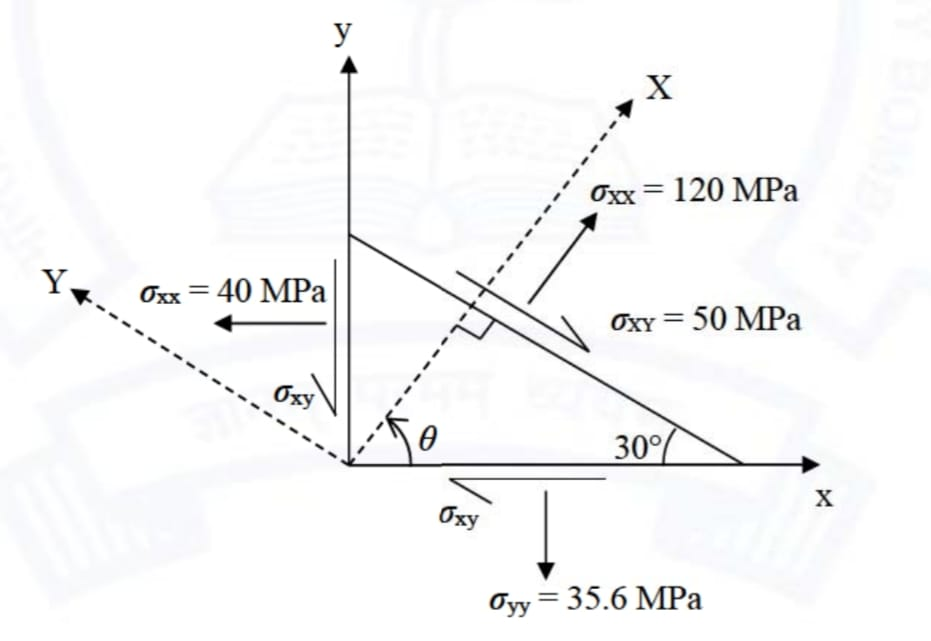
\includegraphics[width=0.7\columnwidth]{figs/1q20.jpg}
    \caption{}
    \label{fig:q20}
\end{figure}
The absolute magnitude of the shear stress component $\sigma_{xy}$ \brak{\text{in MPa, round off to one decimal place}} in x-y coordinate system is \underline{\hspace{2cm}}

\hfill{\brak{\text{GATE CE 2021}}}

\item The equation of deformation is derived to be $y = x^2-xL$ for a beam shown in the figure \figref{fig:q21}
\begin{figure}[H]
    \centering
    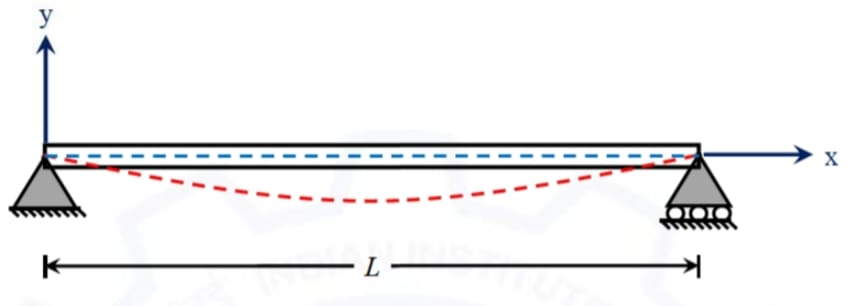
\includegraphics[width=0.7\columnwidth]{figs/1q21.jpg}
    \caption{}
    \label{fig:q21}
\end{figure}
The curvature of the beam at the mid-span \brak{\text{in units, in integer}} will be \underline{\hspace{2cm}}

\hfill{\brak{\text{GATE CE 2021}}}

\item A truss $EFGH$ is shown in the figure \figref{fig:q22}, in which all the members have the same axial rigidity $R$. In the figure, $P$ is the magnitude of external horizontal forces acting at joints F and G.
\begin{figure}[H]
    \centering
    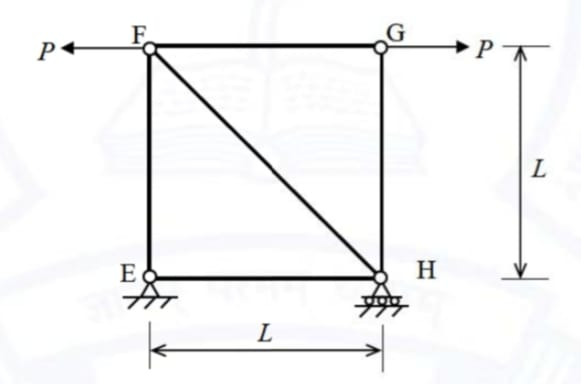
\includegraphics[width=0.7\columnwidth]{figs/1q22.jpg}
    \caption{}
    \label{fig:q22}
\end{figure}
If $R = 500 \times 10^3$ kN, $P = 150$ kN and $L = 3$ m, the magnitude of the horizontal displacement of joint G \brak{\text{in mm, round off to one decimal place}} is \underline{\hspace{2cm}}

\hfill{\brak{\text{GATE CE 2021}}}

\item The cohesion \brak{c}, angle of internal friction \brak{\phi} and unit weight \brak{\gamma} of a soil are 15 kPa, 20$\degree$ and 17.5 kN/m$^3$, respectively. The maximum depth of unsupported excavation in the soil \brak{\text{in m, round off to two decimal places}} is \underline{\hspace{2cm}}

\hfill{\brak{\text{GATE CE 2021}}}

\item Two reservoirs are connected through a homogeneous and isotropic aquifer having hydraulic conductivity \brak{K} of 25 m/day and effective porosity \brak{\eta} of $0.3$ as shown in the figure \figref{fig:q24}  \brak{\text{not to scale}}. Ground water is flowing in the aquifer at the steady state.
\begin{figure}[H]
    \centering
    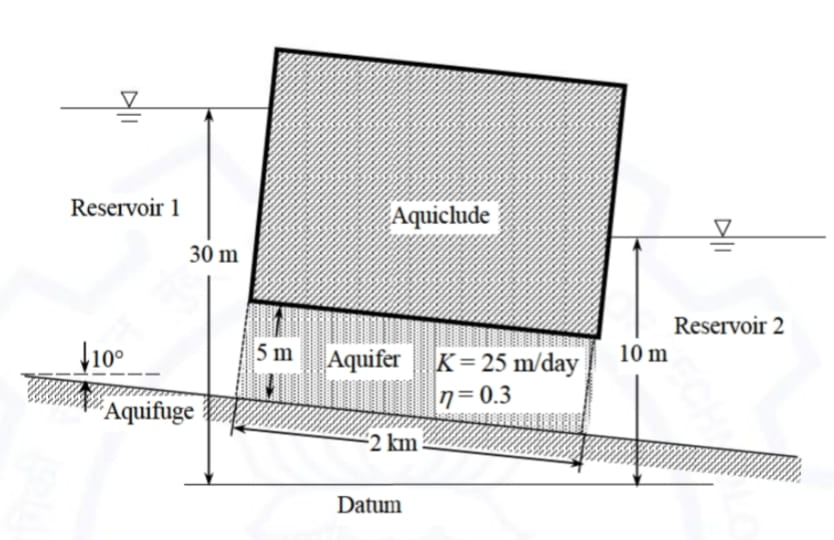
\includegraphics[width=0.7\columnwidth]{figs/1q24.jpg}
    \caption{}
    \label{fig:q24}
\end{figure}
If water in Reservoir 1 is contaminated then the time \brak{\text{in days, round off to one decimal place}} taken by the contaminated water to reach to Reservoir 2 will be \underline{\hspace{2cm}}
\hfill{\brak{\text{GATE CE 2021}}}

\item A signalized intersection operates in two phases. The lost time is $3$ seconds per phase. The maximum ratios of approach flow to saturation flow for the two phases are 0.37 and 0.40. The optimum cycle length using the Webster's method \brak{\text{in seconds, round off to one decimal place}} is \underline{\hspace{2cm}}
\hfill{\brak{\text{GATE CE 2021}}}

\textbf{Q.26 - Q.35 Multiple Choice Question}

\item The solution of the second-order differential equation $\frac{d^2y}{dx^2} + 2\frac{dy}{dx} + y = 0$ with boundary conditions $y\brak{0}=1$ and $y\brak{1}=3$ is

\hfill{\brak{\text{GATE CE 2021}}}
\begin{enumerate}
    \item $e^{-x}+\brak{3e-1}xe^{-x}$
    \item $e^{-x}-\brak{3e-1}xe^{-x}$
    \item $e^{-x} + \sbrak{3e\sin\brak{\frac{\pi x}{2}}-1}xe^{-x}$
    \item $e^{-x} - \sbrak{3e\sin\brak{\frac{\pi x}{2}}-1}xe^{-x}$
\end{enumerate}

\item The value of $\int_0^1 e^x dx$ using the trapezoidal rule with four equal subintervals is

\hfill{\brak{\text{GATE CE 2021}}}
\begin{enumerate}
\begin{multicols}{2}
    \item $1.718$
    \item $1.727$
    \item $2.192$
    \item $2.718$
\end{multicols}
\end{enumerate}

\item A 50 mL sample of industrial wastewater is taken into a silica crucible. The empty weight of the crucible is $54.352$ g. The crucible with the sample is dried in a hot air oven at 104$\degree$C till a constant weight of 55.129 g. Thereafter, the crucible with the dried sample is fired at 600$\degree$C for 1 h in a muffle furnace, and the weight of the crucible along with residue is determined as 54.783 g. The concentration of total volatile solids is \underline{\hspace{2cm}}.

\hfill{\brak{\text{GATE CE 2021}}}
\begin{enumerate}
\begin{multicols}{2}
    \item $15540$ mg/L
    \item $8620$ mg/L
    \item $6920$ mg/L
    \item $1700$ mg/L
\end{multicols}
\end{enumerate}

\item A wedge M and a block N are subjected to forces P and Q as shown in the figure \figref{fig:q29}. If force P is sufficiently large, then the block N can be raised. The weights of the wedge and the block are negligible compared to the forces P and Q. The coefficient of friction \brak{\mu} along the inclined surface between the wedge and the block is $0.2$. All other surfaces are frictionless. The wedge angle is 30$\degree$.
\begin{figure}[H]
    \centering
    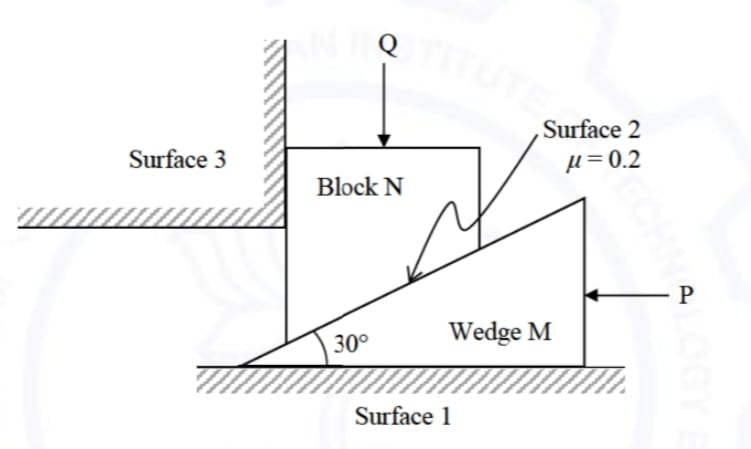
\includegraphics[width=0.7\columnwidth]{figs/1q29.jpg}
    \caption{}
    \label{fig:q29}
\end{figure}
The limiting force P, in terms of Q, required for impending motion of block N to just move it in the upward direction is given as $P = \alpha Q$. The value of the coefficient '$\alpha$' \brak{\text{round off to one decimal place}} is

\hfill{\brak{\text{GATE CE 2021}}}
\begin{enumerate}
\begin{multicols}{4}
    \item 0.6
    \item 0.5
    \item 2.0
    \item 0.9
\end{multicols}
\end{enumerate}

\item Contractor X is developing his bidding strategy against Contractor Y. The ratio of Y's bid price to X's cost for the 30 previous bids in which Contractor X has competed against Contractor Y is given in the Table
\begin{table}[H]
    \centering
    \begin{tabular}{|c|c|}
    \hline
    \textbf{Ratio of Y's bid} & \textbf{Number of} \\
    \textbf{price to X's cost} & \textbf{bids} \\
    \hline
    $1.02$ & $6$ \\
    \hline
    $1.04$ & $12$ \\
    \hline
    $1.06$ & $3$ \\
    \hline
    $1.10$ & $6$ \\
    \hline
    $1.12$ & $3$ \\
    \hline
    \end{tabular}
    \caption{}
    \label{tab:q30}
\end{table}
Based on the bidding behaviour of the Contractor Y, the probability of winning against Contractor Y at a mark up of $8\%$ for the next project is

\hfill{\brak{\text{GATE CE 2021}}}
\begin{enumerate}
    \item $0\%$
    \item more than $0\%$ but less than $50\%$
    \item more than $50\%$ but less than $100\%$
    \item $100\%$
\end{enumerate}

\item Based on drained triaxial shear tests on sands and clays, the representative variations of volumetric strain \brak{\Delta V/V} with the shear strain \brak{\gamma} is shown in the figure \figref{fig:q31}.
\begin{figure}[H]
    \centering
    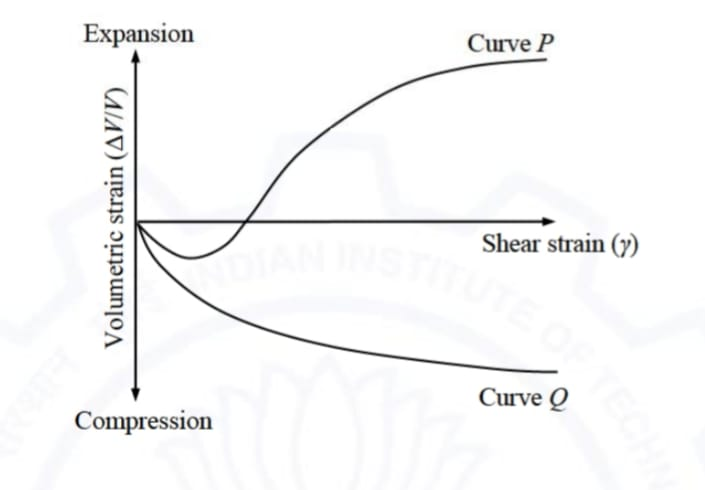
\includegraphics[width=0.7\columnwidth]{figs/1q31.jpg}
    \caption{}
    \label{fig:q31}
\end{figure}
Choose the CORRECT option regarding the representative behaviour exhibited by Curve P and Curve Q.

\hfill{\brak{\text{GATE CE 2021}}}
\begin{enumerate}
    \item Curve P represents dense sand and overconsolidated clay, while Curve Q represents loose sand and normally consolidated clay
    \item Curve P represents dense sand and normally consolidated clay, while Curve Q represents loose sand and overconsolidated clay
    \item Curve P represents loose sand and overconsolidated clay, while Curve Q represents dense sand and normally consolidated clay
    \item Curve P represents loose sand and normally consolidated clay, while Curve Q represents dense sand and overconsolidated clay
\end{enumerate}

\item A fluid flowing steadily in a circular pipe of radius R has a velocity that is everywhere parallel to the axis \brak{\text{centerline}} of the pipe. The velocity distribution along the radial direction is $V_r = U \brak{1-\frac{r^2}{R^2}}$, where r is the radial distance as measured from the pipe axis and U is the maximum velocity at $r=0$. The average velocity of the fluid in the pipe is

\hfill{\brak{\text{GATE CE 2021}}}
\begin{enumerate}
\begin{multicols}{2}
    \item $\frac{U}{2}$
    \item $\frac{U}{3}$
    \item $\frac{U}{4}$
    \item $\brak{\frac{5}{6}}U$
\end{multicols}
\end{enumerate}

\item A water sample is analyzed for coliform organisms by the multiple-tube fermentation method. The results of confirmed test are as follows:
\begin{table}[H]
    \centering
    \begin{tabular}{|c|c|c|}
    \hline
    \textbf{Sample size} & \textbf{Number of positive} & \textbf{Number of negative} \\
    \textbf{\brak{mL}} & \textbf{results out of 5 tubes} & \textbf{results out of 5 tubes} \\
    \hline
    $0.01$ & $5$ & $0$ \\
    \hline
    $0.001$ & $3$ & $2$ \\
    \hline
    $0.0001$ & $1$ & $4$ \\
    \hline
    \end{tabular}
    \caption{}
    \label{tab:q33a}
\end{table}
The most probable number \brak{MPN} of coliform organisms for the above results is to be obtained using the following MPN Index.
\begin{table}[H]
    \centering
    \begin{tabular}{|c|c|}
    \hline
    \multicolumn{2}{|p{8cm}|}{\textbf{MPN Index for Various Combinations of Positive Results when Five Tubes used per Dilution of 10.0 mL, 1.0 mL and 0.1 mL}} \\
    \hline
    \textbf{Combination of positive tubes} & \textbf{MPN Index per 100 mL} \\
    \hline
    $0-2-4$ & $11$ \\
    \hline
    $1-3-5$ & $19$ \\
    \hline
    $4-2-0$ & $22$ \\
    \hline
    $5-3-1$ & $110$ \\
    \hline
    \end{tabular}
    \caption{}
    \label{tab:q33b}
\end{table}
The MPN of coliform organisms per $100$ mL is

\hfill{\brak{\text{GATE CE 2021}}}
\begin{enumerate}
\begin{multicols}{2}
    \item $1100000$
    \item $110000$
    \item $1100$
    \item $110$
\end{multicols}
\end{enumerate}

\item Ammonia nitrogen is present in a given wastewater sample as the ammonium ion \brak{NH_4^+} and ammonia \brak{NH_3}. If pH is the only deciding factor for the proportion of these two constituents, which of the following is a correct statement?

\hfill{\brak{\text{GATE CE 2021}}}
\begin{enumerate}
    \item At pH above $9.25$, only $\text{NH}_4^+$ will be present.
    \item At pH below $9.25$, $\text{NH}_3$ will be predominant.
    \item At pH $7.0$, $\text{NH}_4^+$ and $\text{NH}_3$ will be found in equal measures.
    \item At pH $7.0$, $\text{NH}_4^+$ will be predominant.
\end{enumerate}

\item On a road, the speed-density relationship of a traffic stream is given by $u = 70-0.7k$ \brak{\text{where speed, u, is in km/h and density, k, is in veh/km}}. At the capacity condition, the average time headway will be

\hfill{\brak{\text{GATE CE 2021}}}
\begin{enumerate}
\begin{multicols}{4}
    \item $0.5$ s
    \item $1.0$ s
    \item $1.6$ s
    \item $2.1$ s
\end{multicols}
\end{enumerate}

\textbf{Q.36 - Q.55 Numerical Answer Type}
\item The values of abscissa \brak{x} and ordinate \brak{y} of a curve are as follows:
\begin{table}[H]
    \centering
    \begin{tabular}{|c|c|}
    \hline
    \textbf{X} & \textbf{y} \\
    \hline
    $2.0$ & $5.00$ \\
    \hline
    $2.5$ & $7.25$ \\
    \hline
    $3.0$ & $10.00$ \\
    \hline
    $3.5$ & $13.25$ \\
    \hline
    $4.0$ & $17.00$ \\
    \hline
    \end{tabular}
    \caption{}
    \label{tab:q36}
\end{table}
By Simpson's $1/3^{\text{rd}}$ rule, the area under the curve \brak{\text{round off to two decimal places}} is \underline{\hspace{2cm}}

\hfill{\brak{\text{GATE CE 2021}}}

\item Vehicular arrival at an isolated intersection follows the Poisson distribution. The mean vehicular arrival rate is 2 vehicle per minute. The probability \brak{\text{round off to two decimal places}} that at least $2$ vehicles will arrive in any given $1$-minute interval is \underline{\hspace{2cm}}

\hfill{\brak{\text{GATE CE 2021}}}

\item Refer the truss as shown in the figure \figref{fig:q38} \brak{\text{not to scale}}.
\begin{figure}[H]
    \centering
    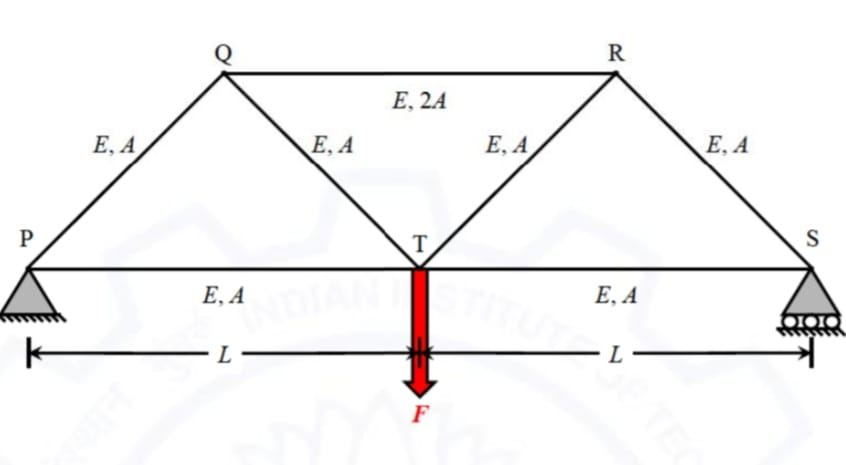
\includegraphics[width=0.7\columnwidth]{figs/1q38.jpg}
    \caption{}
    \label{fig:q38}
\end{figure}
If load, $F = 10\sqrt{3}$ kN, moment of inertia, $I = 8.33 \times 10^6 mm^4$, area of cross-section, $A = 10^4 mm^2$, and length, $L = 2$ m for all the members of the truss, the compressive stress \brak{\text{in kN/m$^2$, in integer}} carried by the member Q-R is \underline{\hspace{2cm}}

\hfill{\brak{\text{GATE CE 2021}}}

\item A prismatic cantilever prestressed concrete beam of span length, $L=1.5$ m has one straight tendon placed in the cross-section as shown in the following figure \figref{fig:q39} . The total prestressing force of $50$ kN in the tendon is applied at $d_c = 50$ mm from the top in the cross-section of width, $b = 200$ mm and depth, $d = 300$ mm.
\begin{figure}[H]
    \centering
    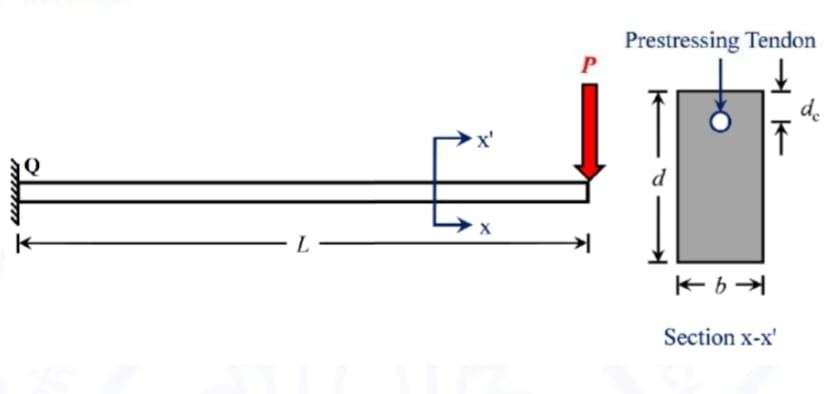
\includegraphics[width=0.7\columnwidth]{figs/1q39.jpg}
    \caption{}
    \label{fig:q39}
\end{figure}
If the concentrated load, $P = 5$ kN, the resultant stress \brak{\text{in MPa, in integer}} experienced at point 'Q' will be \underline{\hspace{2cm}}

\hfill{\brak{\text{GATE CE 2021}}}

\item A column is subjected to a total load \brak{P} of $60$ kN supported through a bracket connection, as shown in the figure \figref{fig:q40}.
\begin{figure}[H]
    \centering
    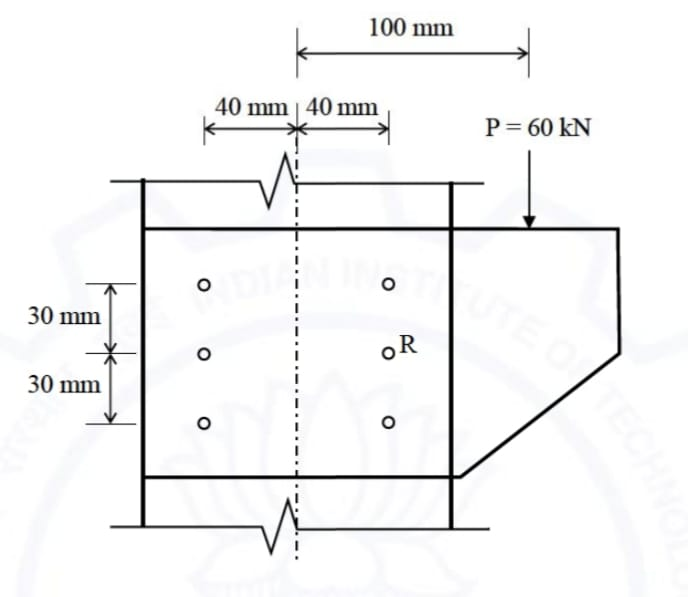
\includegraphics[width=0.7\columnwidth]{figs/1q40.jpg}
    \caption{}
    \label{fig:q40}
\end{figure}
The resultant force in bolt R \brak{\text{in kN, round off to one decimal place}} is \underline{\hspace{2cm}}

\hfill{\brak{\text{GATE CE 2021}}}

\item Employ stiffness matrix approach for the simply supported beam as shown in the figure \figref{fig:q41} to calculate unknown displacements/rotations. Take length, $L=8$ m; modulus of elasticity, $E = 3 \times 10^4 N/mm^2$; moment of inertia, $I = 225 \times 10^6 mm^4$.
\begin{figure}[H]
    \centering
    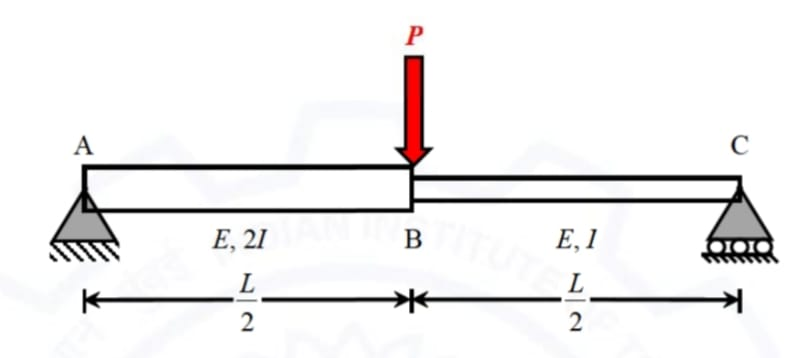
\includegraphics[width=0.7\columnwidth]{figs/1q41.jpg}
    \caption{}
    \label{fig:q41}
\end{figure}
The mid-span deflection of the beam \brak{\text{in mm, round off to integer}} under $P = 100$ kN in downward direction will be \underline{\hspace{2cm}}

\hfill{\brak{\text{GATE CE 2021}}}

\item A square plate O-P-Q-R of a linear elastic material with sides $1.0$ m is loaded in a state of plane stress. Under a given stress condition, the plate deforms to a new configuration O-P'-Q'-R' as shown in the figure \figref{fig:q42}. Under the given deformation, the edges of the plate remain straight.
\begin{figure}[H]
    \centering
    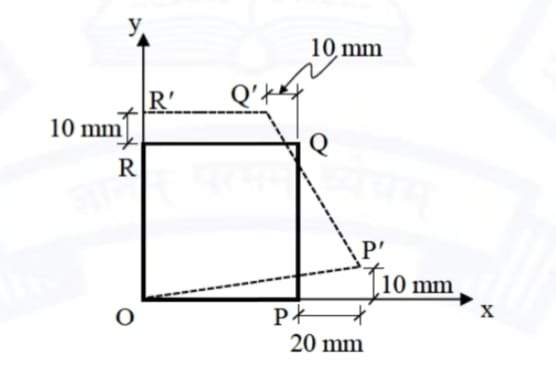
\includegraphics[width=0.7\columnwidth]{figs/1q42.jpg}
    \caption{}
    \label{fig:q42}
\end{figure}
The horizontal displacement of the point \brak{0.5 m, 0.5 m} in the plate O-P-Q-R \brak{\text{in mm, round off to one decimal place}} is \underline{\hspace{2cm}}

\hfill{\brak{\text{GATE CE 2021}}}

\item A small project has $12$ activities - N, P, Q, R, S, T, U, V, W, X, Y, and Z. The relationship among these activities and the duration of these activities are given in the Table.
\begin{table}[H]
    \centering
    \begin{tabular}{|c|c|c|}
    \hline
    \textbf{Activity} & \textbf{Duration} & \textbf{Depends} \\
    & \textbf{\brak{in weeks}} & \textbf{upon} \\
    \hline
    N & $2$ & - \\
    \hline
    P & $5$ & N \\
    \hline
    Q & $3$ & N \\
    \hline
    R & $4$ & P \\
    \hline
    S & $5$ & Q \\
    \hline
    T & $8$ & R \\
    \hline
    U & $7$ & R, S \\
    \hline
    V & $2$ & U \\
    \hline
    W & $3$ & U \\
    \hline
    X & $5$ & T, V \\
    \hline
    Y & $1$ & W \\
    \hline
    Z & $3$ & X, Y \\
    \hline
    \end{tabular}
    \caption{}
    \label{tab:q43}
\end{table}
The total float of the activity "V" \brak{\text{in weeks, in integer}} is \underline{\hspace{2cm}}

\hfill{\brak{\text{GATE CE 2021}}}

\item The soil profile at a construction site is shown in the figure \figref{fig:q44}. Ground water table \brak{GWT} is at $5$ m below the ground level at present. An old well data shows that the ground water table was as low as $10$ m below the ground level in the past. Take unit weight of water, $\gamma_w = 9.81 kN/m^3$.
\begin{figure}[H]
    \centering
    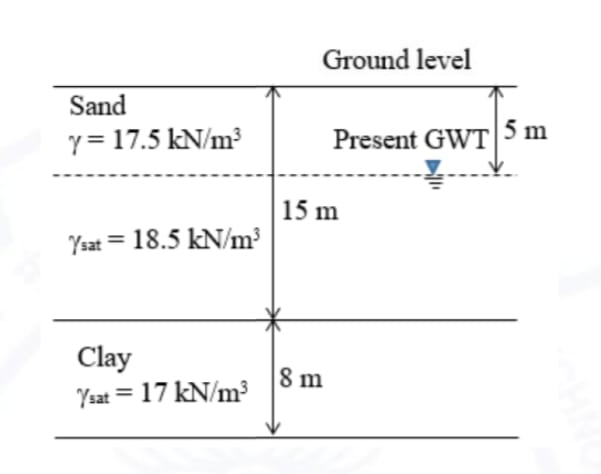
\includegraphics[width=0.7\columnwidth]{figs/1q44.jpg}
    \caption{}
    \label{fig:q44}
\end{figure}
The overconsolidation ratio \brak{OCR} \brak{\text{round off to two decimal places}} at the mid-point of the clay layer is \underline{\hspace{2cm}}

\hfill{\brak{\text{GATE CE 2021}}}

\item A retaining wall of height $10$ m with clay backfill is shown in the figure \figref{fig:q45}. Weight of the retaining wall is $5000$ kN per m acting at $3.3$ m from the toe of the retaining wall. The interface friction angle between base of the retaining wall and the base soil is $20\degree$. The depth of clay in front of the retaining wall is $2.0$ m. The properties of the clay backfill and the clay placed in front of the retaining wall are the same. Assume that the tension crack is filled with water. Use Rankine's earth pressure theory. Take unit weight of water, $\gamma_w = 9.81 kN/m^3$.
\begin{figure}[H]
    \centering
    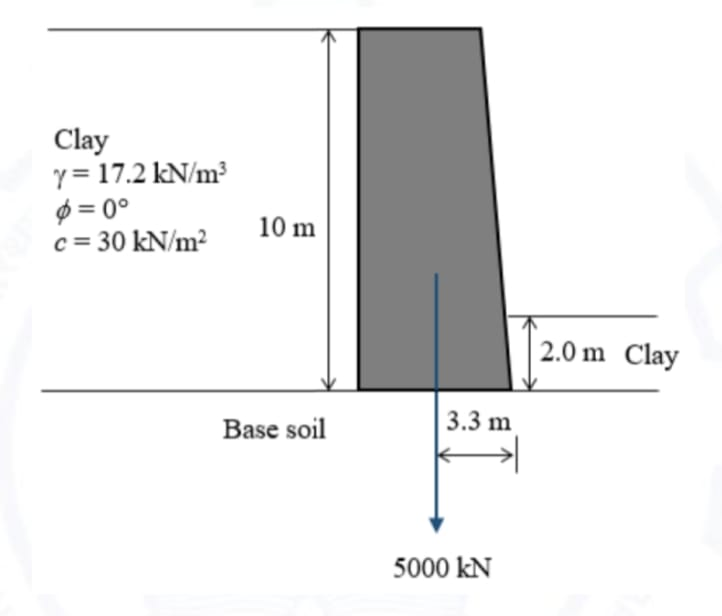
\includegraphics[width=0.7\columnwidth]{figs/1q45.jpg}
    \caption{}
    \label{fig:q45}
\end{figure}
The factor of safety \brak{\text{round off to two decimal places}} against sliding failure of the retaining wall after ignoring the passive earth pressure will be \underline{\hspace{2cm}}

\hfill{\brak{\text{GATE CE 2021}}}

\item A combined trapezoidal footing of length L supports two identical square columns \brak{\text{$P_1$ and $P_2$}} of size $0.5 m \times 0.5 m$, as shown in the figure \figref{fig:q45} . The columns $P_1$ and $P_2$ carry loads of $2000$ kN and $1500$ kN, respectively.
\begin{figure}[H]
    \centering
    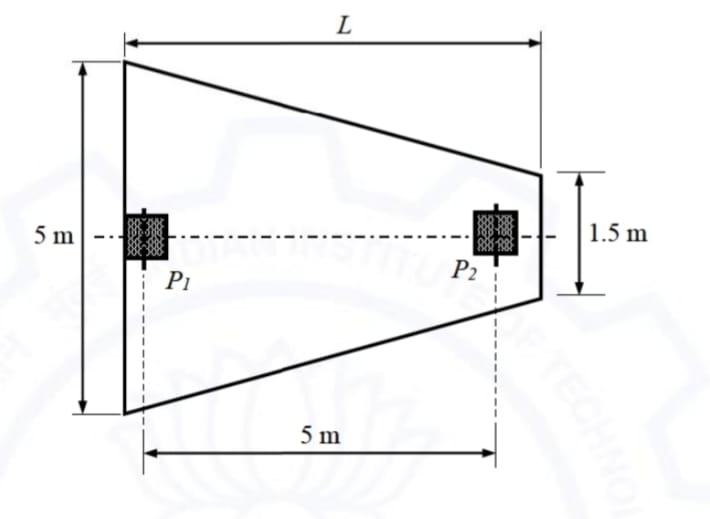
\includegraphics[width=0.7\columnwidth]{figs/1q46.jpg}
    \caption{}
    \label{fig:q46}
\end{figure}
If the stress beneath the footing is uniform, the length of the combined footing L \brak{\text{in m, round off to two decimal places}} is \underline{\hspace{2cm}}

\hfill{\brak{\text{GATE CE 2021}}}

\item An unsupported slope of height 15 m is shown in the figure \figref{fig:q47}, in which the slope face makes an angle $50\degree$ with the horizontal. The slope material comprises purely cohesive soil having undrained cohesion 75 kPa. A trial slip circle KLM, with a radius 25 m, passes through the crest and toe of the slope and it subtends an angle $60\degree$ at its center O. The weight of the active soil mass \brak{\text{W, bounded by KLMN}} is 2500 kN/m, which is acting at a horizontal distance of 10 m from the toe of the slope. Consider the water table to be present at a very large depth from the ground surface.
\begin{figure}[H]
    \centering
    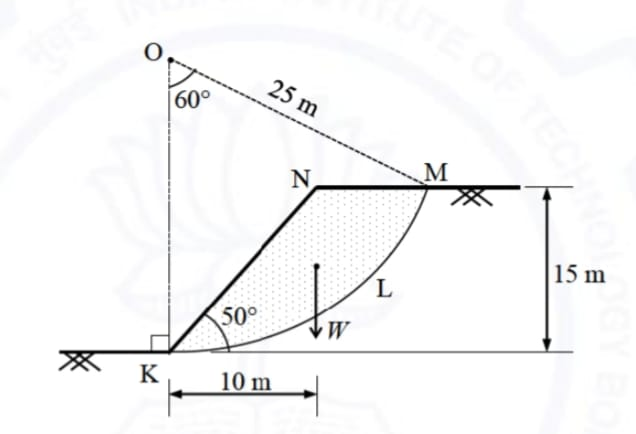
\includegraphics[width=0.7\columnwidth]{figs/1q47.jpg}
    \caption{}
    \label{fig:q47}
\end{figure}
Considering the trial slip circle KLM, the factor of safety against the failure of slope under undrained condition \brak{\text{round off to two decimal places}} is \underline{\hspace{2cm}}

\hfill{\brak{\text{GATE CE 2021}}}

\item An unlined canal under regime conditions along with a silt factor of $1$ has a width of flow $71.25$ m. Assuming the unlined canal as a wide channel, the corresponding average depth of flow \brak{\text{in m, round off to two decimal places}} in the canal will be \underline{\hspace{2cm}}

\hfill{\brak{\text{GATE CE 2021}}}

\item A cylinder \brak{\text{2.0 m diameter, 3.0 m long and 25 kN weight}} is acted upon by water on one side and oil \brak{\text{specific gravity = 0.8}} on other side as shown in the figure \figref{fig:q49}.
\begin{figure}[H]
    \centering
    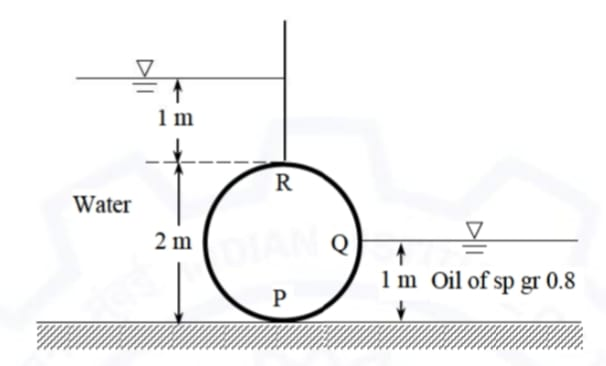
\includegraphics[width=0.7\columnwidth]{figs/1q49.jpg}
    \caption{}
    \label{fig:q49}
\end{figure}
The absolute ratio of the net magnitude of vertical forces to the net magnitude of horizontal forces \brak{\text{round off to two decimal places}} is \underline{\hspace{2cm}}

\hfill{\brak{\text{GATE CE 2021}}}

\item A tube-well of $20$ cm diameter fully penetrates a horizontal, homogeneous and isotropic confined aquifer of infinite horizontal extent. The aquifer is of $30$ m uniform thickness. A steady pumping at the rate of $40$ litres/s from the well for a long time results in a steady drawdown of $4$ m at the well face. The subsurface flow to the well due to pumping is steady, horizontal and Darcian and the radius of influence of the well is $245$ m. The hydraulic conductivity of the aquifer \brak{\text{in m/day, round off to integer}} is \underline{\hspace{2cm}}

\hfill{\brak{\text{GATE CE 2021}}}

\item A baghouse filter has to treat 12 m$^3$/s of waste gas continuously. The baghouse is to be divided into $5$ sections of equal cloth area such that one section can be shut down for cleaning and/or repairing, while the other $4$ sections continue to operate. An air-to-cloth ratio of 6.0 m$^3$/min-m$^2$ cloth will provide sufficient treatment to the gas. The individual bags are of $32$ cm in diameter and $5$ m in length. The total number of bags \brak{\text{in integer}} required in the baghouse is \underline{\hspace{2cm}}

\hfill{\brak{\text{GATE CE 2021}}}

\item A secondary clarifier handles a total flow of 9600 m$^3$/d from the aeration tank of a conventional activated-sludge treatment system. The concentration of solids in the flow from the aeration tank is $3000$ mg/L. The clarifier is required to thicken the solids to $12000$ mg/L, and hence it is to be designed for a solid flux of $3.2 \frac{kg}{m^2 \cdot h}$. The surface area of the designed clarifier for thickening \brak{\text{in m$^2$, in integer}} is \underline{\hspace{2cm}}

\hfill{\brak{\text{GATE CE 2021}}}

\item Spot speeds of vehicles observed at a point on a highway are $40, 55, 60, 65$ and $80$ km/h. The space-mean speed \brak{\text{in km/h, round off to two decimal places}} of the observed vehicles is \underline{\hspace{2cm}}

\hfill{\brak{\text{GATE CE 2021}}}

\item The longitudinal section of a runway provides the following data:
\begin{table}[H]
    \centering
    \begin{tabular}{|c|c|}
    \hline
    \textbf{End-to-end runway \brak{m}} & \textbf{Gradient \brak{\%}} \\
    \hline
    $0$ to $300$ & $+1.2$ \\
    \hline
    $300$ to $600$ & $-0.7$ \\
    \hline
    $600$ to $1100$ & $+0.6$ \\
    \hline
    $1100$ to $1400$ & $-0.8$ \\
    \hline
    $1400$ to $1700$ & $-1.0$ \\
    \hline
    \end{tabular}
    \caption{}
    \label{tab:q54}
\end{table}
The effective gradient of the runway \brak{\text{in \%, round off to two decimal places}} is \underline{\hspace{2cm}}

\hfill{\brak{\text{GATE CE 2021}}}

\item Traversing is carried out for a closed traverse PQRS. The internal angles at vertices P, Q, R and S are measured as 92$\degree$, 68$\degree$, 123$\degree$, and 77$\degree$, respectively. If fore bearing of line PQ is 27$\degree$, fore bearing of line RS \brak{\text{in degrees, in integer}} is \underline{\hspace{2cm}}

\hfill{\brak{\text{GATE CE 2021}}}

\end{enumerate}




\textbf{SESSION - 2}
\section*{Q.1 - Q.5 Multiple Choice Question carry one mark each}

\begin{enumerate}
\item 
\begin{enumerate}
    \item[\brak{i}] Arun and Aparna are here.
    \item[\brak{ii}] Arun and Aparna is here.
    \item[\brak{iii}] Arun's families is here.
    \item[\brak{iv}] Arun's family is here.
\end{enumerate}
Which of the above sentences are grammatically CORRECT?

\hfill{\brak{\text{GATE CE 2021}}}

\begin{multicols}{2}
\begin{enumerate}
    \item \brak{i} and \brak{ii}
    \item \brak{i} and \brak{iv}
    \item \brak{ii} and \brak{iv}
    \item \brak{iii} and \brak{iv}
\end{enumerate}
\end{multicols}

\item The mirror image of the above text about the x-axis is
\begin{figure}[H]
    \centering
    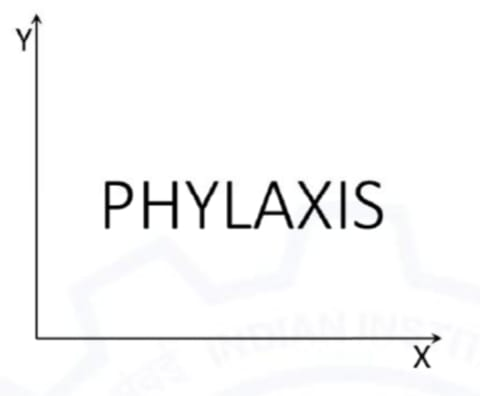
\includegraphics[width=0.7\columnwidth]{figs/2q2.jpg}
    \caption{}
    \label{fig:q2}
\end{figure}
\begin{multicols}{2}
\begin{enumerate}
    \item \begin{figure}[H]
    \centering
    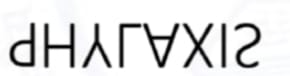
\includegraphics[width=0.5\columnwidth]{figs/2q2a.jpg}
    \caption{}
    \label{fig:q2}
\end{figure}
\item \begin{figure}[H]
    \centering
    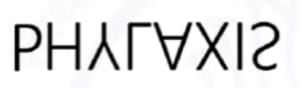
\includegraphics[width=0.5\columnwidth]{figs/2q2b.jpg}
    \caption{}
    \label{fig:q2}
\end{figure}
\item \begin{figure}[H]
    \centering
    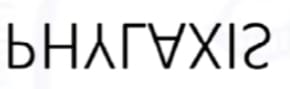
\includegraphics[width=0.5\columnwidth]{figs/2q2c.jpg}
    \caption{}
    \label{fig:q2}
\end{figure}
\item \begin{figure}[H]
    \centering
    
\includegraphics[width=0.5\columnwidth]{figs/2q2d.jpg}
    \caption{}
    \label{fig:q2}
\end{figure}
\end{enumerate}
\end{multicols}
\hfill{\brak{\text{GATE CE 2021}}}



\item Two identical cube shaped dice each with faces numbered 1 to 6 are rolled simultaneously. The probability that an even number is rolled out on each dice is:

\hfill{\brak{\text{GATE CE 2021}}}
\begin{multicols}{4}
\begin{enumerate}
    \item $\frac{1}{36}$
    \item $\frac{1}{12}$
    \item $\frac{1}{8}$
    \item $\frac{1}{4}$
\end{enumerate}
\end{multicols}

\item $\odot$ and $\oplus$ are two operators on numbers $p$ and $q$ such that
$p \odot q = p - q$, and $p \oplus q = p \times q$
Then, $\brak{9 \odot \brak{6 \oplus 7}} \odot \brak{7 \oplus \brak{6 \odot 5}} = $

\hfill{\brak{\text{GATE CE 2021}}}

\begin{multicols}{2}
\begin{enumerate}
    \item $40$
    \item $-26$
    \item $-33$
    \item $-40$
\end{enumerate}
\end{multicols}

\item Four persons P, Q, R and S are to be seated in a row. R should not be seated at the second position from the left end of the row. The number of distinct seating arrangements possible is:

\hfill{\brak{\text{GATE CE 2021}}}

\begin{multicols}{2}
\begin{enumerate}
    \item $6$
    \item $9$
    \item $18$
    \item $24$
\end{enumerate}
\end{multicols}

\textbf{Q.6 - Q.10 Multiple Choice Question carry two mark each}

\item On a planar field, you travelled 3 units East from a point O. Next you travelled 4 units South to arrive at point P. Then you travelled from P in the North-East direction such that you arrive at a point that is 6 units East of point O. Next, you travelled in the North-West direction, so that you arrive at point Q that is 8 units North of point P.
The distance of point Q to point O, in the same units, should be \underline{\hspace{2cm}}

\hfill{\brak{\text{GATE CE 2021}}}

\begin{multicols}{2}
\begin{enumerate}
    \item $3$
    \item $4$
    \item $5$
    \item $6$
\end{enumerate}
\end{multicols}

\item The author said, "Musicians rehearse before their concerts. Actors rehearse their roles before the opening of a new play. On the other hand, I find it strange that many public speakers think they can just walk on to the stage and start speaking. In my opinion, it is no less important for public speakers to rehearse their talks."
Based on the above passage, which one of the following is TRUE?

\hfill{\brak{\text{GATE CE 2021}}}

\begin{enumerate}
    \item The author is of the opinion that rehearsing is important for musicians, actors and public speakers.
    \item The author is of the opinion that rehearsing is less important for public speakers than for musicians and actors.
    \item The author is of the opinion that rehearsing is more important only for musicians than public speakers.
    \item The author is of the opinion that rehearsal is more important for actors than musicians.
\end{enumerate}

\item 
1. Some football players play cricket.

2. All cricket players play hockey.

Among the options given below, the statement that logically follows from the two statements 1 and 2 above, is:

\hfill{\brak{\text{GATE CE 2021}}}

\begin{enumerate}
    \item No football player plays hockey.
    \item Some football players play hockey.
    \item All football players play hockey.
    \item All hockey players play football.
\end{enumerate}

\item In the figure \figref{fig:q9} shown above, $PQRS$ is a square. The shaded portion is formed by the intersection of sectors of circles with radius equal to the side of the square and centers at $S$ and $Q$.
The probability that any point picked randomly within the square falls in the shaded area is \underline{\hspace{2cm}}
\begin{figure}[H]
    \centering
    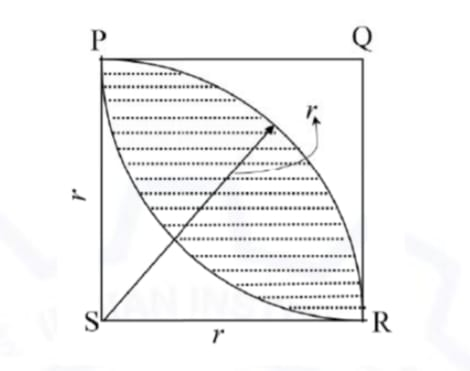
\includegraphics[width=0.7\columnwidth]{figs/2q9.jpg}
    \caption{}
    \label{fig:q9}
\end{figure}

\hfill{\brak{\text{GATE CE 2021}}}

\begin{multicols}{2}
\begin{enumerate}
    \item $4-\frac{\pi}{2}$
    \item $\frac{1}{2}$
    \item $\frac{\pi}{2}-1$
    \item $\frac{\pi}{4}$
\end{enumerate}
\end{multicols}

\item In an equilateral triangle $PQR$, side $PQ$ is divided into four equal parts, side $QR$ is divided into six equal parts and side $PR$ is divided into eight equal parts. The length of each subdivided part in cm is an integer.
The minimum area of the triangle $PQR$ possible, in cm$^2$, is

\hfill{\brak{\text{GATE CE 2021}}}

\begin{multicols}{2}
\begin{enumerate}
    \item 18
    \item 24
    \item $48\sqrt{3}$
    \item $144\sqrt{3}$
\end{enumerate}
\end{multicols}
\end{enumerate}

\textbf{Q.1 - Q.16 Multiple Choice Question carry one mark each }

\begin{enumerate}
\item The value of $\lim_{x \to \infty} \frac{x \ln\brak{x}}{1+x^2}$ is

\hfill{\brak{\text{GATE CE 2021}}}

\begin{multicols}{2}
\begin{enumerate}
    \item 0
    \item 1.0
    \item 0.5
    \item $\infty$
\end{enumerate}
\end{multicols}

\item The rank of the matrix $\myvec{5 & 0 & -5 & 0 \\ 0 & 2 & 0 & 1 \\ -5 & 0 & 5 & 0 \\ 0 & 1 & 0 & 2}$ is

\hfill{\brak{\text{GATE CE 2021}}}

\begin{multicols}{2}
\begin{enumerate}
    \item 1
    \item 2
    \item 3
    \item 4
\end{enumerate}
\end{multicols}

\item The unit normal vector to the surface $X^2+Y^2+Z^2-48=0$ at the point $\brak{4, 4, 4}$ is

\hfill{\brak{\text{GATE CE 2021}}}

\begin{enumerate}
    \item $\frac{1}{\sqrt{2}}, \frac{1}{\sqrt{2}}, \frac{1}{\sqrt{2}}$
    \item $\frac{1}{\sqrt{3}}, \frac{1}{\sqrt{3}}, \frac{1}{\sqrt{3}}$
    \item $\frac{2}{\sqrt{2}}, \frac{2}{\sqrt{2}}, \frac{2}{\sqrt{2}}$
    \item $\frac{1}{\sqrt{5}}, \frac{1}{\sqrt{5}}, \frac{1}{\sqrt{5}}$
\end{enumerate}

\item If A is a square matrix then orthogonality property mandates

\hfill{\brak{\text{GATE CE 2021}}}

\begin{multicols}{2}
\begin{enumerate}
    \item $AA^T = I$
    \item $AA^T = 0$
    \item $AA^T = A^{-1}$
    \item $AA^T = A^2$
\end{enumerate}
\end{multicols}

\item In general, the CORRECT sequence of surveying operations is

\hfill{\brak{\text{GATE CE 2021}}}

\begin{enumerate}
    \item Field observations $\rightarrow$ Reconnaissance $\rightarrow$ Data analysis $\rightarrow$ Map making
    \item Data analysis $\rightarrow$ Reconnaissance $\rightarrow$ Field observations $\rightarrow$ Map making
    \item Reconnaissance $\rightarrow$ Field observations $\rightarrow$ Data analysis $\rightarrow$ Map making
    \item Reconnaissance $\rightarrow$ Data analysis $\rightarrow$ Field observations $\rightarrow$ Map making
\end{enumerate}

\item Strain hardening of structural steel means

\hfill{\brak{\text{GATE CE 2021}}}

\begin{enumerate}
    \item experiencing higher stress than yield stress with increased deformation
    \item strengthening steel member externally for reducing strain experienced
    \item strain occurring before plastic flow of steel material
    \item decrease in the stress experienced with increasing strain
\end{enumerate}

\item A single story building model is shown in the figure \figref{fig:q7}. The rigid bar of mass 'm' is supported by three massless elastic columns whose ends are fixed against rotation. For each of the columns, the applied lateral force $\brak{P}$ and corresponding moment $\brak{M}$ are also shown in the figure. The lateral deflection $\brak{\delta}$ of the bar is given by $\delta = \frac{PL^3}{12EI}$, where $L$ is the effective length of the column, $E$ is the Young's modulus of elasticity and $I$ is the area moment of inertia of the column cross-section with respect to its neutral axis.
\begin{figure}[H]
    \centering
    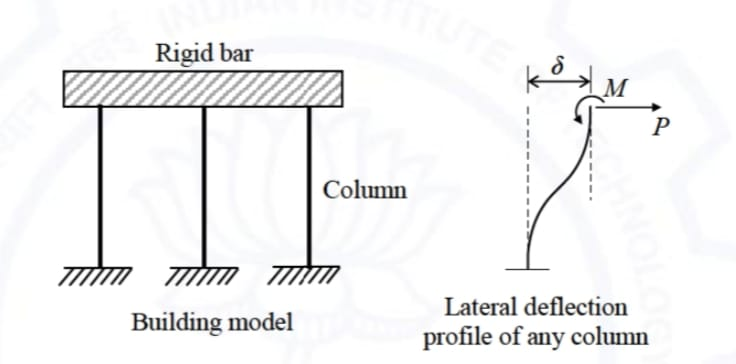
\includegraphics[width=0.7\columnwidth]{figs/2q7.jpg}
    \caption{}
    \label{fig:q7}
\end{figure}
For the lateral deflection profile of the columns as shown in the figure \figref{fig:q7}, the natural frequency of the system for horizontal oscillation is

\hfill{\brak{\text{GATE CE 2021}}}

\begin{enumerate}
    \item $6 \sqrt{\frac{EI}{mL^3}}$ rad/s
    \item $\frac{1}{L} \sqrt{\frac{2EI}{m}}$ rad/s
    \item $2 \sqrt{\frac{6EI}{mL^3}}$ rad/s
    \item $\frac{2}{L} \sqrt{\frac{EI}{m}}$ rad/s
\end{enumerate}

\item Seasoning of timber for use in construction is done essentially to

\hfill{\brak{\text{GATE CE 2021}}}

\begin{enumerate}
    \item increase strength and durability
    \item smoothen timber surfaces
    \item remove knots from timber logs
    \item cut timber in right season and geometry
\end{enumerate}

\item In case of bids in Two-Envelop System, the correct option is

\hfill{\brak{\text{GATE CE 2021}}}

\begin{enumerate}
    \item Technical bid is opened first
    \item Financial bid is opened first
    \item Both \brak{\text{Technical and Financial}} bids are opened simultaneously
    \item Either of the two \brak{\text{Technical and Financial}} bids can be opened first
\end{enumerate}

\item The most appropriate triaxial test to assess the long-term stability of an excavated clay slope is

\hfill{\brak{\text{GATE CE 2021}}}

\begin{enumerate}
    \item consolidated drained test
    \item unconsolidated undrained test
    \item consolidated undrained test
    \item unconfined compression test
\end{enumerate}

\item As per the Unified Soil Classification System $\brak{USCS}$, the type of soil represented by 'MH' is

\hfill{\brak{\text{GATE CE 2021}}}

\begin{enumerate}
    \item Inorganic silts of high plasticity with liquid limit more than 50\%
    \item Inorganic silts of low plasticity with liquid limit less than 50\%
    \item Inorganic clays of high plasticity with liquid limit less than 50\%
    \item Inorganic clays of low plasticity with liquid limit more than 50\%
\end{enumerate}

\item The ratio of the momentum correction factor to the energy correction factor for a laminar flow in a pipe is

\hfill{\brak{\text{GATE CE 2021}}}

\begin{multicols}{2}
\begin{enumerate}
    \item $\frac{1}{2}$
    \item $\frac{2}{3}$
    \item $1$
    \item $\frac{3}{2}$
\end{enumerate}
\end{multicols}

\item Relationship between traffic speed and density is described using a negatively sloped straight line. If $v_f$ is the free-flow speed then the speed at which the maximum flow occurs is

\hfill{\brak{\text{GATE CE 2021}}}

\begin{multicols}{2}
\begin{enumerate}
    \item $0$
    \item $\frac{v_f}{4}$
    \item $\frac{v_f}{2}$
    \item $v_f$
\end{enumerate}
\end{multicols}

\item Determine the correctness or otherwise of the following Assertion \sbrak{a} and the Reason \sbrak{r}.

Assertion \sbrak{a}: One of the best ways to reduce the amount of solid wastes is to reduce the consumption of raw materials.

Reason \sbrak{r}: Solid wastes are seldom generated when raw materials are converted to goods for consumption.

\hfill{\brak{\text{GATE CE 2021}}}

\begin{enumerate}
    \item Both \sbrak{a} and \sbrak{r} are true and \sbrak{r} is the correct reason for \sbrak{a}
    \item Both \sbrak{a} and \sbrak{r} are true but \sbrak{r} is not the correct reason for \sbrak{a}
    \item Both \sbrak{a} and \sbrak{r} are false
    \item the \sbrak{a} is true but \sbrak{r} is false
\end{enumerate}

\item The hardness of a water sample is measured directly by titration with 0.01 M solution of ethylenediamine tetraacetic acid $\brak{EDTA}$ using eriochrome black T $\brak{EBT}$ as an indicator. The EBT reacts and forms complexes with divalent metallic cations present in the water. During titration, the EDTA replaces the EBT in the complex. When the replacement of EBT is complete at the end point of the titration, the colour of the solution changes from

\hfill{\brak{\text{GATE CE 2021}}}

\begin{enumerate}
    \item blue-green to reddish brown
    \item blue to colourless
    \item reddish brown to pinkish yellow
    \item wine red to blue
\end{enumerate}

\item The softening point of bitumen has the same unit as that of

\hfill{\brak{\text{GATE CE 2021}}}

\begin{multicols}{2}
\begin{enumerate}
    \item distance
    \item temperature
    \item time
    \item viscosity
\end{enumerate}
\end{multicols}

\textbf{ Q.17 Multiple Select Question }
\item Which of the following statement is/are correct?

\hfill{\brak{\text{GATE CE 2021}}}

\begin{enumerate}
    \item Increased levels of carbon monoxide in the indoor environment result in the formation of carboxyhemoglobin and the long term exposure becomes a cause of cardiovascular diseases.
    \item Volatile organic compounds act as one of the precursors to the formation of photochemical smog in the presence of sunlight.
    \item Long term exposure to the increased level of photochemical smog becomes a cause of chest constriction and irritation of the mucous membrane.
    \item Increased levels of volatile organic compounds in the indoor environment will result in the formation of photochemical smog which is a cause of cardiovascular diseases.
\end{enumerate}

\textbf{Q.18 - Q.25 Numerical Answer Question }
\item The value $\brak{\text{round off to one decimal place}}$ of $\int_{-1}^{1} x e^{\abs{x}} dx$ is \underline{\hspace{2cm}}

\hfill{\brak{\text{GATE CE 2021}}}

\item A solid circular torsional member OPQ is subjected to torsional moments as shown in the figure \figref{fig:q19} $\brak{\text{not to scale}}$. The yield shear strength of the constituent material is 160 MPa.
\begin{figure}[H]
    \centering
    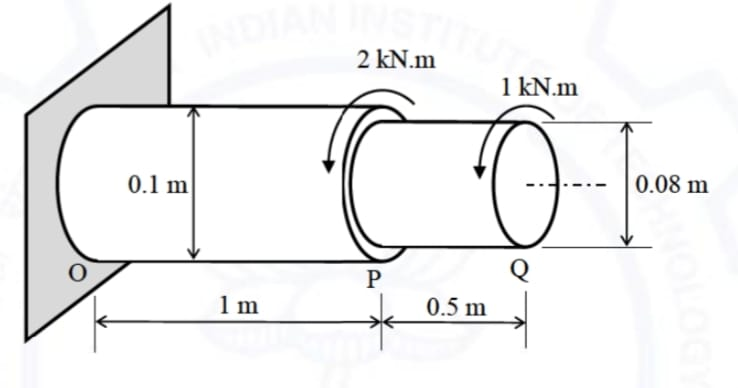
\includegraphics[width=0.7\columnwidth]{figs/2q19.jpg}
    \caption{}
    \label{fig:q19}
\end{figure}
The absolute maximum shear stress in the member $\brak{\text{in MPa, round off to one decimal place}}$ is \underline{\hspace{2cm}}

\hfill{\brak{\text{GATE CE 2021}}}

\item A propped cantilever beam XY, with an internal hinge at the middle, is carrying a uniformly distributed load of 10 kN/m, as shown in the figure \figref{fig:q20}.
\begin{figure}[H]
    \centering
    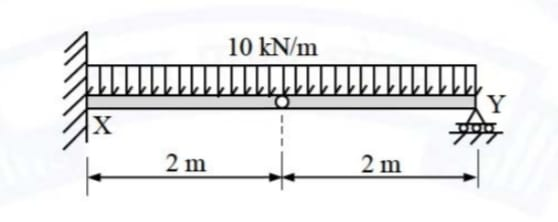
\includegraphics[width=0.7\columnwidth]{figs/2q20.jpg}
    \caption{}
    \label{fig:q20}
\end{figure}
The vertical reaction at support X $\brak{\text{in kN, in integer}}$ is \underline{\hspace{2cm}}

\hfill{\brak{\text{GATE CE 2021}}}

\item The internal $\brak{d_i}$ and external $\brak{d_o}$ diameters of a Shelby sampler are 48 mm and 52 mm, respectively. The area ratio $\brak{A_r}$ of the sampler $\brak{\text{in \%, round off to two decimal places}}$ is \underline{\hspace{2cm}}

\hfill{\brak{\text{GATE CE 2021}}}

\item A 12-hour unit hydrograph $\brak{\text{of 1 cm excess rainfall}}$ of a catchment is of a triangular shape with a base width of 144 hour and a peak discharge of 23 m$^3$/s. The area of the catchment \brak{\text{in km$^2$, round off to the nearest integer}} is \underline{\hspace{2cm}}

\hfill{\brak{\text{GATE CE 2021}}}

\item A lake has a maximum depth of 60 m. If the mean atmospheric pressure in the lake region is 91 kPa and the unit weight of the lake water is 9790 N/m$^3$, the absolute pressure $\brak{\text{in kPa, round off to two decimal places}}$ at the maximum depth of the lake is \underline{\hspace{2cm}}

\hfill{\brak{\text{GATE CE 2021}}}

\item In a three-phase signal system design for a four-leg intersection, the critical flow ratios for each phase are 0.18, 0.32, and 0.22. The total loss time in each of the phases is 2 s. As per Webster's formula, the optimal cycle length \brak{\text{in s, round off to the nearest integer}} is \underline{\hspace{2cm}}

\hfill{\brak{\text{GATE CE 2021}}}

\item A horizontal angle $\theta$ is measured by four different surveyors multiple times and the values reported are given below.
\begin{table}[H]
    \centering
    \begin{tabular}{|c|c|c|}
        \hline
        \textbf{Surveyor} & \textbf{Angle $\theta$} & \textbf{Number of observations} \\ \hline
        1 & $36\degree30'$ & 4 \\ \hline
        2 & $36\degree00'$ & 3 \\ \hline
        3 & $35\degree30'$ & 8 \\ \hline
        4 & $36\degree30'$ & 4 \\ \hline
    \end{tabular}
    \caption{}
    \label{tab:q25}
\end{table}
The most probable value of the angle $\theta$ \brak{\text{in degree, round off to two decimal places}} is \underline{\hspace{2cm}}

\hfill{\brak{\text{GATE CE 2021}}}

\textbf{Q.26 - Q.35 Multiple Choice Questions}
\item If $k$ is a constant, the general solution of $\frac{dy}{dx} - \frac{y}{x} = 1$ will be in the form of

\hfill{\brak{\text{GATE CE 2021}}}

\begin{multicols}{2}
\begin{enumerate}
    \item $y = x\ln\brak{kx}$
    \item $y = k\ln\brak{kx}$
    \item $y = x\ln\brak{x}$
    \item $y = xk\ln\brak{k}$
\end{enumerate}
\end{multicols}

\item The smallest eigenvalue and the corresponding eigenvector of the matrix $\myvec{2 & -2 \\ -1 & 6}$, respectively, are

\hfill{\brak{\text{GATE CE 2021}}}

\begin{enumerate}
    \item 1.55 and $\myvec{2.00 \\ 0.45}$
    \item 2.00 and $\myvec{1.00 \\ 1.00}$
    \item 1.55 and $\myvec{-2.55 \\ -0.45}$
    \item 1.55 and $\myvec{2.00 \\ -0.45}$
\end{enumerate}

\item A prismatic steel beam is shown in the figure \figref{fig:q28} .
\begin{figure}[H]
    \centering
    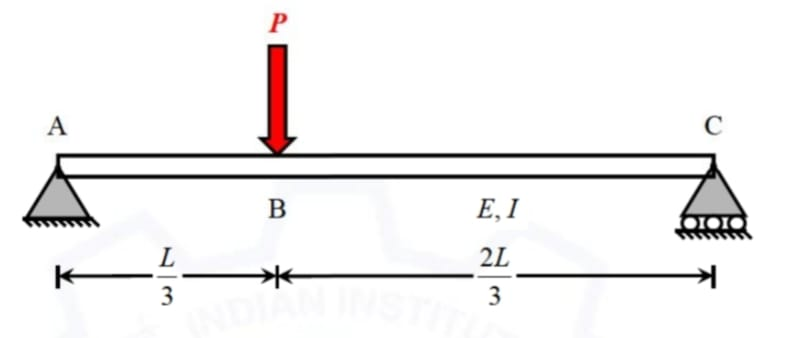
\includegraphics[width=0.7\columnwidth]{figs/2q28.jpg}
    \caption{}
    \label{fig:q28}
\end{figure}
The plastic moment, $M_p$ calculated for the collapse mechanism using static method and kinematic method is

\hfill{\brak{\text{GATE CE 2021}}}

\begin{enumerate}
    \item $M_{p,static} > \frac{2PL}{9} = M_{p,kinematic}$
    \item $M_{p,static} = \frac{2PL}{9} \ne M_{p,kinematic}$
    \item $M_{p,static} = \frac{2PL}{9} = M_{p,kinematic}$
    \item $M_{p,static} < \frac{2PL}{9} = M_{p,kinematic}$
\end{enumerate}

\item A frame EFG is shown in the figure \figref{fig:q29} . All members are prismatic and have equal flexural rigidity. The member FG carries a uniformly distributed load w per unit length. Axial deformation of any member is neglected.
\begin{figure}[H]
    \centering
    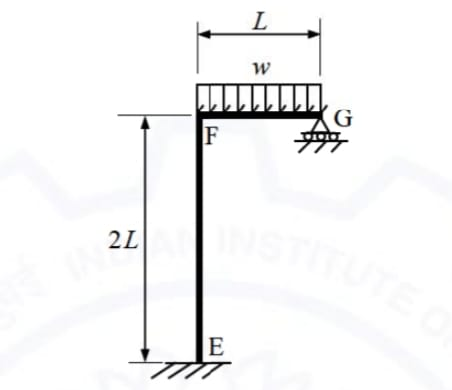
\includegraphics[width=0.7\columnwidth]{figs/2q29.jpg}
    \caption{}
    \label{fig:q29}
\end{figure}
Considering the joint F being rigid, the support reaction at G is

\hfill{\brak{\text{GATE CE 2021}}}

\begin{multicols}{2}
\begin{enumerate}
    \item $0.375 wL$
    \item $0.453 wL$
    \item $0.482 wL$
    \item $0.500 wL$
\end{enumerate}
\end{multicols}

\item A clay layer of thickness $H$ has a preconsolidation pressure $p_c$ and an initial void ratio $e_0$. The initial effective overburden stress at the mid-height of the layer is $p_0$. At the same location, the increment in effective stress due to applied external load is $\Delta p$. The compression and swelling indices of the clay are $C_c$ and $C_s$, respectively. If $p_0 < p_c < \brak{p_0 + \Delta p}$, then the correct expression to estimate the consolidation settlement $\brak{s_c}$ of the clay layer is

\hfill{\brak{\text{GATE CE 2021}}}

\begin{enumerate}
    \item $s_c = \frac{H}{1+e_0} \sbrak{ C_c \log \frac{p_c}{p_0} + C_s \log \frac{p_0+\Delta p}{p_c} }$
    \item $s_c = \frac{H}{1+e_0} \sbrak{ C_s \log \frac{p_c}{p_0} + C_c \log \frac{p_0+\Delta p}{p_c} }$
    \item $s_c = \frac{H}{1+e_0} \sbrak{ C_c \log \frac{p_0}{p_c} + C_s \log \frac{p_0+\Delta p}{p_c} }$
    \item $s_c = \frac{H}{1+e_0} \sbrak{C_s \log \frac{p_0}{p_c} + C_c \log \frac{p_0+\Delta p}{p_c} }$
\end{enumerate}

\item A rectangular open channel of 6 m width is carrying a discharge of 20 m$^3$/s. Consider the acceleration due to gravity as 9.81 m/s$^2$ and assume water as incompressible and inviscid. The depth of flow in the channel at which the specific energy of the flowing water is minimum for the given discharge will then be

\hfill{\brak{\text{GATE CE 2021}}}

\begin{multicols}{2}
\begin{enumerate}
    \item 0.82 m
    \item 1.04 m
    \item 2.56 m
    \item 3.18 m
\end{enumerate}
\end{multicols}

\item Read the statements given below.
\begin{enumerate}
    \item[\brak{i}] Value of the wind profile exponent for the 'very unstable' atmosphere is smaller than the wind profile exponent for the 'neutral' atmosphere.
    \item[\brak{ii}] Downwind concentration of air pollutants due to an elevated point source will be inversely proportional to the wind speed.
    \item[\brak{iii}] Value of the wind profile exponent for the 'neutral' atmosphere is smaller than the wind profile exponent for the 'very unstable' atmosphere.
    \item[\brak{iv}] Downwind concentration of air pollutants due to an elevated point source will be directly proportional to the wind speed.
\end{enumerate}
Select the correct option.

\hfill{\brak{\text{GATE CE 2021}}}

\begin{enumerate}
    \item \brak{i} is False and \brak{iii} is True
    \item \brak{i} is True and \brak{iv} is True
    \item \brak{ii} is False and \brak{iii} is False
    \item \brak{iii} is False and \brak{iv} is False
\end{enumerate}

\item A water filtration unit is made of uniform-size sand particles of 0.4 mm diameter with a shape factor of 0.84 and specific gravity of 2.55. The depth of the filter bed is 0.70 m and the porosity is 0.35. The filter bed is to be expanded to a porosity of 0.65 by hydraulic backwash. If the terminal settling velocity of sand particles during backwash is 4.5 cm/s, the required backwash velocity is

\hfill{\brak{\text{GATE CE 2021}}}

\begin{multicols}{2}
\begin{enumerate}
    \item $5.79 \times 10^{-3}$ m/s
    \item $6.35 \times 10^{-3}$ m/s
    \item 0.69 cm/s
    \item 0.75 cm/s
\end{enumerate}
\end{multicols}

\item For a given traverse, latitudes and departures are calculated and it is found that sum of latitudes is equal to +2.1 m and the sum of departures is equal to -2.8 m. The length and bearing of the closing error, respectively, are

\hfill{\brak{\text{GATE CE 2021}}}

\begin{multicols}{2}
\begin{enumerate}
    \item 3.50 m and $53\degree7'48"$ NW
    \item 2.45 m and $53\degree7'48"$ NW
    \item 0.35 m and $53.13\degree$ SE
    \item 3.50 m and $53.13\degree$ SE
\end{enumerate}
\end{multicols}

\item From laboratory investigations, the liquid limit, plastic limit, natural moisture content and flow index of a soil specimen are obtained as 60\%, 27\%, 32\% and 27, respectively. The corresponding toughness index and liquidity index of the soil specimen, respectively, are

\hfill{\brak{\text{GATE CE 2021}}}

\begin{multicols}{2}
\begin{enumerate}
    \item 0.15 and 1.22
    \item 0.19 and 6.60
    \item 1.22 and 0.15
    \item 6.60 and 0.19
\end{enumerate}
\end{multicols}

\textbf{Numerical Answer Questions}
\item A function is defined in Cartesian coordinate system as $f\brak{x,y} = xe^y$. The value of the directional derivative of the function $\brak{\text{in integer}}$ at the point $\brak{2, 0}$ along the direction of the straight line segment from point $\brak{2, 0}$ to point $\brak{\frac{1}{2}, 2}$ is \underline{\hspace{2cm}}

\hfill{\brak{\text{GATE CE 2021}}}

\item An elevated cylindrical water storage tank is shown in the figure \figref{fig:q37}. The tank has inner diameter of 1.5 m. It is supported on a solid steel circular column of diameter 75 mm and total height $\brak{L}$ of 4 m. Take, water density = 1000 kg/m$^3$ and acceleration due to gravity = 10 m/s$^2$.
\begin{figure}[H]
    \centering
    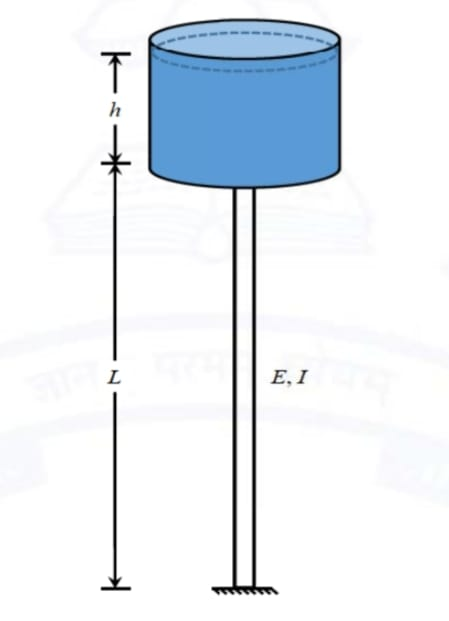
\includegraphics[width=0.7\columnwidth]{figs/2q37.jpg}
    \caption{}
    \label{fig:q37}
\end{figure}
If elastic modulus $\brak{E}$ of steel is 200 GPa, ignoring self-weight of the tank, for the supporting steel column to remain unbuckled, the maximum depth $\brak{h}$ of the water permissible $\brak{\text{in m, round off to one decimal place}}$ is \underline{\hspace{2cm}}

\hfill{\brak{\text{GATE CE 2021}}}

\item A prismatic fixed-fixed beam, modelled with a total lumped-mass of 10 kg as a single degree of freedom $\brak{SDOF}$ system is shown in the figure \figref{fig:q38}.
\begin{figure}[H]
    \centering
    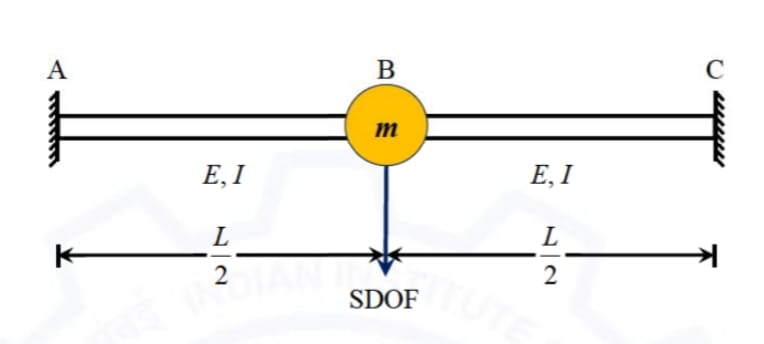
\includegraphics[width=0.7\columnwidth]{figs/2q38.jpg}
    \caption{}
    \label{fig:q38}
\end{figure}
If the flexural stiffness of the beam is $4\pi^2$ kN/m, its natural frequency of vibration $\brak{\text{in Hz, in integer}}$ in the flexural mode will be \underline{\hspace{2cm}}

\hfill{\brak{\text{GATE CE 2021}}}

\item A perfectly flexible and inextensible cable is shown in the figure \figref{fig:q39} $\brak{\text{not to scale}}$. The external loads at F and G are acting vertically.
\begin{figure}[H]
    \centering
    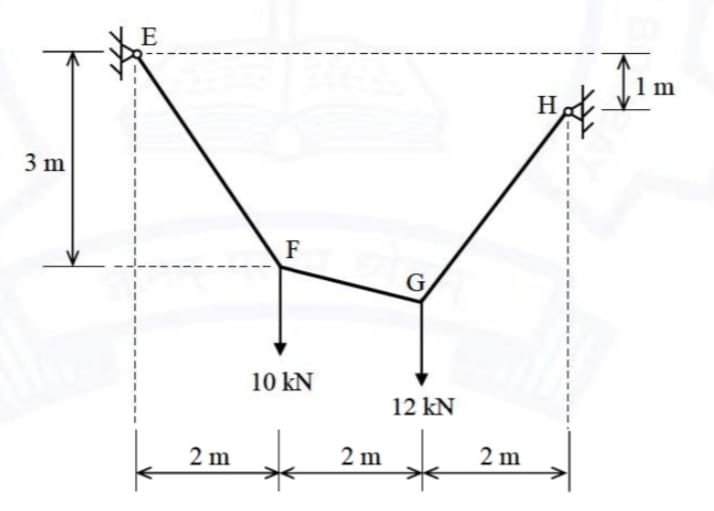
\includegraphics[width=0.7\columnwidth]{figs/2q39.jpg}
    \caption{}
    \label{fig:q39}
\end{figure}
The magnitude of tension in the cable segment FG $\brak{\text{in kN, round off to two decimal places}}$ is \underline{\hspace{2cm}}

\hfill{\brak{\text{GATE CE 2021}}}

\item A fire hose nozzle directs a steady stream of water of velocity 50 m/s at an angle of 45$\degree$ above the horizontal. The stream rises initially but then eventually falls to the ground. Assume water as incompressible and inviscid. Consider the density of air and the air friction as negligible, and assume the acceleration due to gravity as 9.81 m/s$^2$. The maximum height $\brak{\text{in m, round off to two decimal places}}$ reached by the stream above the hose nozzle will then be \underline{\hspace{2cm}}

\hfill{\brak{\text{GATE CE 2021}}}

\item A rectangular cross-section of a reinforced concrete beam is shown in the figure \figref{fig:q41}. The diameter of each reinforcing bar is 16 mm. The values of modulus of elasticity of concrete and steel are $2.0 \times 10^4$ MPa and $2.1 \times 10^5$ MPa, respectively.
\begin{figure}[H]
    \centering
    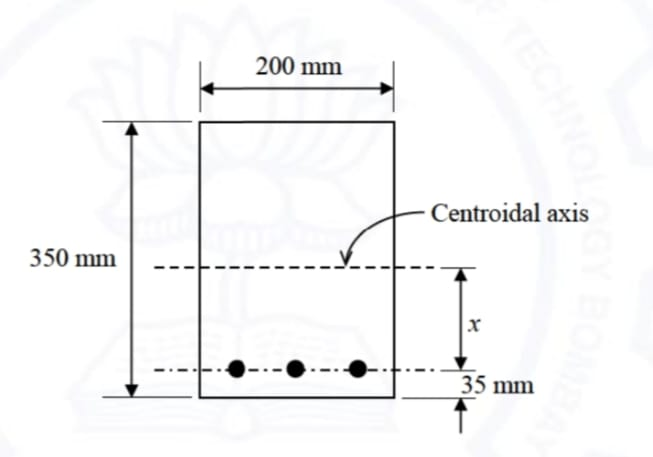
\includegraphics[width=0.7\columnwidth]{figs/2q41.jpg}
    \caption{}
    \label{fig:q41}
\end{figure}
The distance of the centroidal axis from the centerline of the reinforcement $\brak{x}$ for the uncracked section $\brak{\text{in mm, round off to one decimal place}}$ is \underline{\hspace{2cm}}

\hfill{\brak{\text{GATE CE 2021}}}

\item The activity details for a small project are given in the Table.
\begin{table}[H]
    \centering
    \begin{tabular}{|c|c|c|}
        \hline
        \textbf{Activity} & \textbf{Duration (days)} & \textbf{Depends on} \\ \hline
        A & 6 & - \\ \hline
        B & 10 & A \\ \hline
        C & 14 & A \\ \hline
        D & 8 & B \\ \hline
        E & 12 & C \\ \hline
        F & 8 & C \\ \hline
        G & 16 & D, E \\ \hline
        H & 8 & F, G \\ \hline
        K & 2 & B \\ \hline
        L & 5 & G, K \\ \hline
    \end{tabular}
    \caption{}
    \label{tab:q42}
\end{table}
The total time $\brak{\text{in days, in integer}}$ for project completion is \underline{\hspace{2cm}}

\hfill{\brak{\text{GATE CE 2021}}}

\item An equipment has been purchased at an initial cost of Rs.160000 and has an estimated salvage value of Rs.10000. The equipment has an estimated life of 5 years. The difference between the book values $\brak{\text{in Rs, in integer}}$ obtained at the end of 4th year using straight line method and sum of years digit method of depreciation is \underline{\hspace{2cm}}

\hfill{\brak{\text{GATE CE 2021}}}

\item A rectangular footing of size 2.8 m $\times$ 3.5 m is embedded in a clay layer and a vertical load is placed with an eccentricity of 0.8 m as shown in the figure \figref{fig:q44} $\brak{\text{not to scale}}$. Take Bearing capacity factors: $N_c = 5.14, N_q = 1.0$, and $N_{\gamma} = 0.0$; Shape factors: $s_c = 1.16, s_q = 1.0$ and $s_{\gamma}= 1.0$; Depth factors: $d_c = 1.1, d_q = 1.0$ and $d_{\gamma} = 1.0$; and Inclination factors: $i_c = 1.0$ and $i_q = 1.0$ and $i_{\gamma}= 1.0$.
\begin{figure}[H]
    \centering
    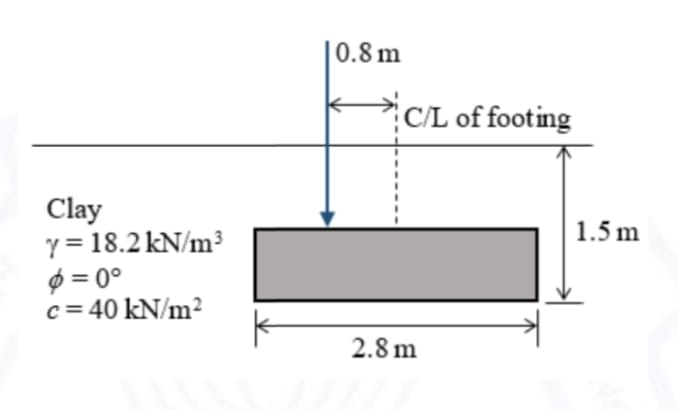
\includegraphics[width=0.7\columnwidth]{figs/2q44.jpg}
    \caption{}
    \label{fig:q44}
\end{figure}
Using Meyerhoff's method, the load $\brak{\text{in kN, round off to two decimal places}}$ that can be applied on the footing with a factor of safety of 2.5 is \underline{\hspace{2cm}}

\hfill{\brak{\text{GATE CE 2021}}}

\item The soil profile at a road construction site is as shown in figure \figref{fig:q45} $\brak{\text{not to scale}}$. A large embankment is to be constructed at the site. The ground water table $\brak{GWT}$ is located at the surface of the clay layer, and the capillary rise in the sandy soil is negligible. The effective stress at the middle of the clay layer after the application of the embankment loading is 180 kN/m$^2$. Take unit weight of water, $\gamma_w = 9.81$ kN/m$^3$.
\begin{figure}[H]
    \centering
    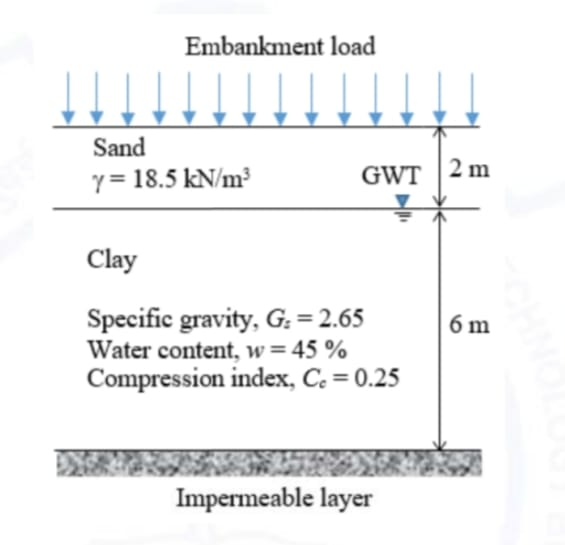
\includegraphics[width=0.7\columnwidth]{figs/2q45.jpg}
    \caption{}
    \label{fig:q45}
\end{figure}
The primary consolidation settlement \brak{\text{in m, round off to two decimal places}} of the clay layer resulting from this loading will be \underline{\hspace{2cm}}

\hfill{\brak{\text{GATE CE 2021}}}

\item Numerically integrate, $f\brak{x} = 10x - 20x^2$ from lower limit $a = 0$ to upper limit $b = 0.5$. Use Trapezoidal rule with five equal subdivisions. The value $\brak{\text{in units, round off to two decimal places}}$ obtained is \underline{\hspace{2cm}}

\hfill{\brak{\text{GATE CE 2021}}}

\item The void ratio of a clay soil sample M decreased from 0.575 to 0.510 when the applied pressure is increased from 120 kPa to 180 kPa. For the same increment in pressure, the void ratio of another clay soil sample N decreases from 0.600 to 0.550. If the ratio of hydraulic conductivity of sample M to sample N is 0.125, then the ratio of coefficient of consolidation of sample M to sample N $\brak{\text{round off to three decimal places}}$ is \underline{\hspace{2cm}}

\hfill{\brak{\text{GATE CE 2021}}}

\item The hyetograph in the figure \figref{fig:q48} corresponds to a rainfall event of 3 cm.
\begin{figure}[H]
    \centering
    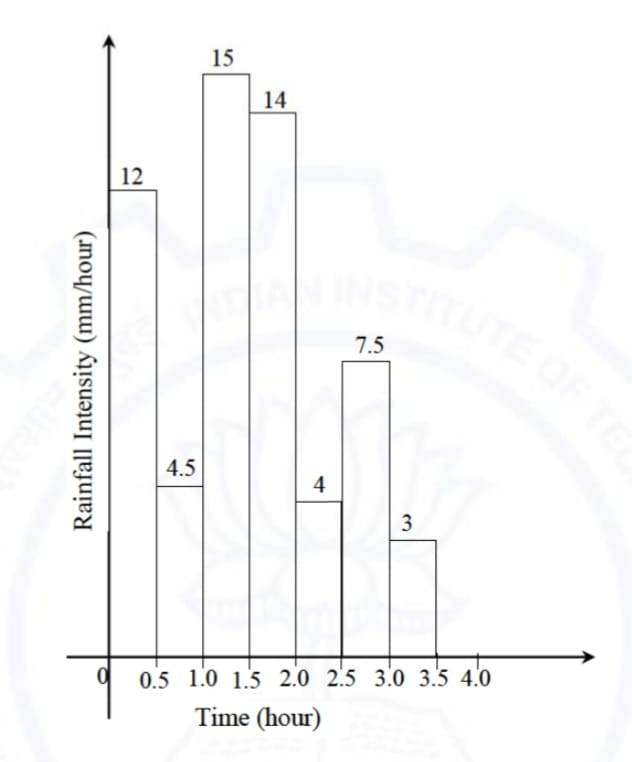
\includegraphics[width=0.7\columnwidth]{figs/2q48.jpg}
    \caption{}
    \label{fig:q48}
\end{figure}
If the rainfall event has produced a direct runoff of 1.6 cm, the $\phi$-index of the event $\brak{\text{in mm/hour, round off to one decimal place}}$ would be \underline{\hspace{2cm}}

\hfill{\brak{\text{GATE CE 2021}}}

\item A venturimeter as shown in the figure \figref{fig:q49} $\brak{\text{not to scale}}$ is connected to measure the flow of water in a vertical pipe of 20 cm diameter.
\begin{figure}[H]
    \centering
    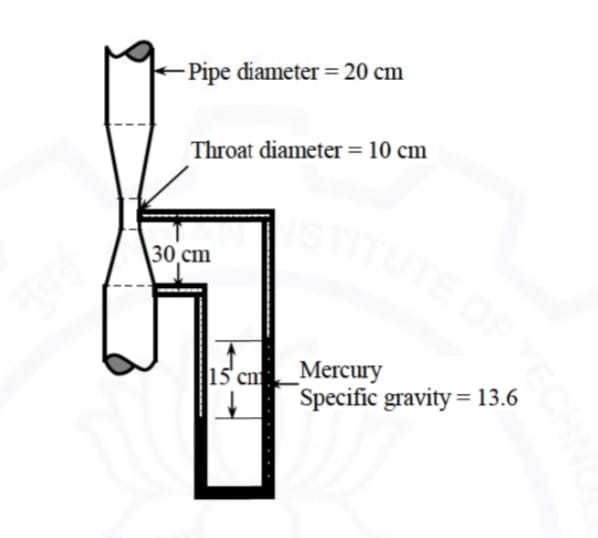
\includegraphics[width=0.7\columnwidth]{figs/2q49.jpg}
    \caption{}
    \label{fig:q49}
\end{figure}
Assume $g = 9.8$ m/s$^2$. When the deflection in the mercury manometer is 15 cm, the flow rate $\brak{\text{in lps, round off to two decimal places}}$ considering no loss in the venturimeter is \underline{\hspace{2cm}}

\hfill{\brak{\text{GATE CE 2021}}}

\item A reservoir with a live storage of 300 million cubic metre irrigates 40000 hectares $\brak{\text{1 hectare} = 10^4 \text{ m}^2}$ of a crop with two fillings of the reservoir. If the base period of the crop is 120 days, 
the duty for this crop \\
$\brak{\text{in hectares per cumec, round off to integer}}$ will then be \underline{\hspace{2cm}}

\hfill{\brak{\text{GATE CE 2021}}}

\item An activated sludge process $\brak{ASP}$ is designed for secondary treatment of 7500 m$^3$/day of municipal wastewater. After primary clarifier, the ultimate BOD of the influent, which enters into ASP reactor is 200 mg/L. Treated effluent after secondary clarifier is required to have an ultimate BOD of 20 mg/L. Mix liquor volatile suspended solids $\brak{MLVSS}$ concentration in the reactor and the underflow is maintained as 3000 mg/L and 12000 mg/L, respectively. The hydraulic retention time and mean cell residence time are 0.2 day and 10 days, respectively. A representative flow diagram of the ASP is shown below \figref{fig:q51}.
\begin{figure}[H]
    \centering
    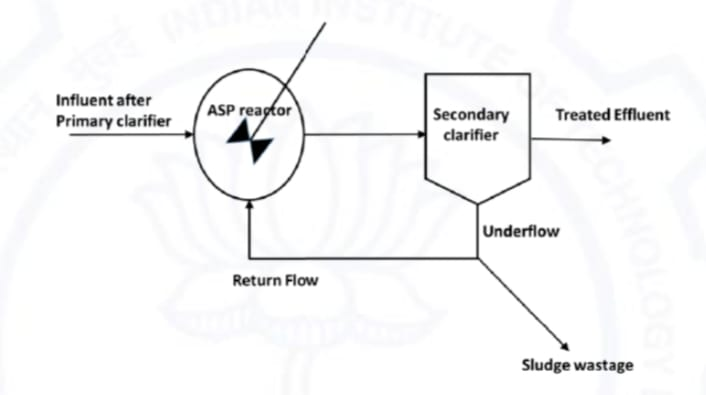
\includegraphics[width=0.7\columnwidth]{figs/2q51.jpg}
    \caption{}
    \label{fig:q51}
\end{figure}
The underflow volume $\brak{\text{in m}^3\text{/day, round off to one decimal place}}$ of sludge wastage is \underline{\hspace{2cm}}

\hfill{\brak{\text{GATE CE 2021}}}

\item A grit chamber of rectangular cross-section is to be designed to remove particles with diameter of 0.25 mm and specific gravity of 2.70. The terminal settling velocity of the particles is estimated as 2.5 cm/s. The chamber is having a width of 0.50 m and has to carry a peak wastewater flow of 9720 m$^3$/d giving the depth of flow as 0.75 m. If a flow-through velocity of 0.3 m/s has to be maintained using a proportional weir at the outlet end of the chamber, the minimum length of the chamber $\brak{\text{in m, in integer}}$ to remove 0.25 mm particles completely is \underline{\hspace{2cm}}

\hfill{\brak{\text{GATE CE 2021}}}

\item In an aggregate mix, the proportions of coarse aggregate, fine aggregate and mineral filler are 55\%, 40\% and 5\%, respectively. The values of bulk specific gravity of the coarse aggregate, fine aggregate and mineral filler are 2.55, 2.65 and 2.70, respectively. The bulk specific gravity of the aggregate mix $\brak{\text{round off to two decimal places}}$ is \underline{\hspace{2cm}}

\hfill{\brak{\text{GATE CE 2021}}}

\item The stopping sight distance $\brak{SSD}$ for a level highway is 140 m for the design speed of 90 km/h. The acceleration due to gravity and deceleration rate are 9.81 m/s$^2$ and 3.5 m/s$^2$, respectively. The perception/reaction time $\brak{\text{in s, round off to two decimal places}}$ used in the $SSD$ calculation is \underline{\hspace{2cm}}

\hfill{\brak{\text{GATE CE 2021}}}

\item For a 2$\degree$ curve on a high speed Broad Gauge $\brak{BG}$ rail section, the maximum sanctioned speed is 100 km/h and the equilibrium speed is 80 km/h. Consider dynamic gauge of BG rail as 1750 mm. The degree of curve is defined as the angle subtended at its center by a 30.5 m arc. The cant deficiency for the curve $\brak{\text{in mm, round off to integer}}$ is \underline{\hspace{2cm}}

\hfill{\brak{\text{GATE CE 2021}}}

\end{enumerate}

\end{document}
